
\documentclass[a4paper
               ,10pt
               ,DIV=10 % Satzspiegel berechnen
               ,BCOR=0.3cm
               ,pagesize % Papiergröße an DVI und PDF übergeben
               %,oneside
               ,headings=small
               ,bibtotoc
               ]
               {scrartcl}

%\parskip 0.3cm

%\usepackage{epsfig,afterpage}
%\usepackage{amsfonts}
\usepackage{amssymb}

%%usepackage{dsfont}

%\usepackage[utf8]{inputenc}

%\usepackage{a4}
%\usepackage{longtable}
%\usepackage{indentfirst}
%\usepackage{verbatim}
\usepackage{amsmath}
\usepackage{amsthm}
\usepackage[pdftex]{graphicx}
\usepackage[ngerman]{babel}
%\usepackage[ngerman,english]{babel}
%\usepackage[latin1]{inputenc}
\usepackage[T1]{fontenc}
%\usepackage{appendix}

\usepackage{caption}
\usepackage{subcaption}
\usepackage{wrapfig}
\usepackage{hyperref}

\usepackage{index}
\makeindex
\hypersetup{%
pdftitle = {Hardware software co design: Legocar}, pdfauthor = {},
linkbordercolor = 0 0 0, pdfborder = 0 0 0, colorlinks = false,
hyperindex=true }


%\selectlanguage{ngerman}
%\usepackage{mathptmx}
%\usepackage[scaled=.90]{helvet}
%\usepackage{courier}
% Schrift
\usepackage{lmodern}
%\usepackage{mathpazo} % Palatino

\usepackage{listings}
\lstloadlanguages{Matlab}
\lstset{language=Matlab,frame=single,numberstyle=\tiny,numbers=left,breaklines=true,tabsize=4,basicstyle=\tiny}

\usepackage{setspace}
\usepackage{psfrag}
\usepackage{graphicx}
%\usepackage[dvips]{graphicx,color}

\usepackage{listings}
\usepackage{color}

\usepackage{placeins}
 
\definecolor{dkgreen}{rgb}{0,0.6,0}
\definecolor{gray}{rgb}{0.5,0.5,0.5}
\definecolor{mauve}{rgb}{0.58,0,0.82}

\lstset{ %
  language=C++,                % the language of the code
  basicstyle=\scriptsize,           % the size of the fonts that are used for the code
  numbers=left,                   % where to put the line-numbers
  numberstyle=\tiny\color{gray},  % the style that is used for the line-numbers
  stepnumber=1,                   % the step between two line-numbers. If it's 1, each line 
                                  % will be numbered
  numbersep=5pt,                  % how far the line-numbers are from the code
  backgroundcolor=\color{white},      % choose the background color. You must add \usepackage{color}
  showspaces=false,               % show spaces adding particular underscores
  showstringspaces=false,         % underline spaces within strings
  showtabs=false,                 % show tabs within strings adding particular underscores
  frame=single,                   % adds a frame around the code
  rulecolor=\color{black},        % if not set, the frame-color may be changed on line-breaks within not-black text (e.g. commens (green here))
  tabsize=2,                      % sets default tabsize to 2 spaces
  captionpos=b,                   % sets the caption-position to bottom
  breaklines=true,                % sets automatic line breaking
  breakatwhitespace=false,        % sets if automatic breaks should only happen at whitespace
  %title=\lstname,                   % show the filename of files included with \lstinputlisting;
                                  % also try caption instead of title
  keywordstyle=\color{blue},          % keyword style
  commentstyle=\color{dkgreen},       % comment style
  stringstyle=\color{mauve},         % string literal style
  escapeinside={\%*}{*)},            % if you want to add LaTeX within your code
  morekeywords={*,...}               % if you want to add more keywords to the set
}

\onehalfspacing


\newtheorem{defn}{Definition}
\newtheorem{thm}{Theorem}
\newtheorem{exmp}{Example}
\newtheorem{rem}{Remark}
\newtheorem{cor}{Corollary}

\graphicspath{{pic/}}

%\usepackage{ifthen}




%\usepackage{dsfont}

%\usepackage{moreverb}
\usepackage{epsfig}
%\usepackage{setspace}

\usepackage{float}

\title{Hardware software co design: Legocar}%%TODO
\author{Wenwen Chen, Christian Dietz, \\
	Jan Seeger, Rainer Schoenberger, Julian Tatsch
}
\date{\today}


\begin{document}
\maketitle

\begin{abstract}
%%TODO
\end{abstract}
\tableofcontents
%----------------------------------------------------------------------------------------
\section{Introduction}
%----------------------------------------------------------------------------------------
\subsection{Overview}

The general architecture of our project is shown in Figure~\ref{figarchitecture}.
The FPGA plays the central role:
It controls the Servo/Motor-controller board and reads the sensor inputs.
In future it can also be connected to a camera.
Due to the limited time we could not implement the camera interface.
The FPGA is also responsible for calculating the current speed based on the sensor inputs and for controlling the motor acceleration.

All the high-level communication is done by the RaspberryPi, which is connected to the FPGA.
It receives steering commands from mobile phones, notebooks or Wiimotes and passes them to the FPGA.
The Raspi creates an Wifi access point and has a bluetooth interface.
This way, any Wifi and TCP/IP capable device as well as Wiimote controllers can control the car.

Besides the real hardware, there exists a software simulator for the car.
It has the same interface as the RaspberryPi and can be used to simulate steering algorithms.

\begin{figure}[H]
\begin{center}
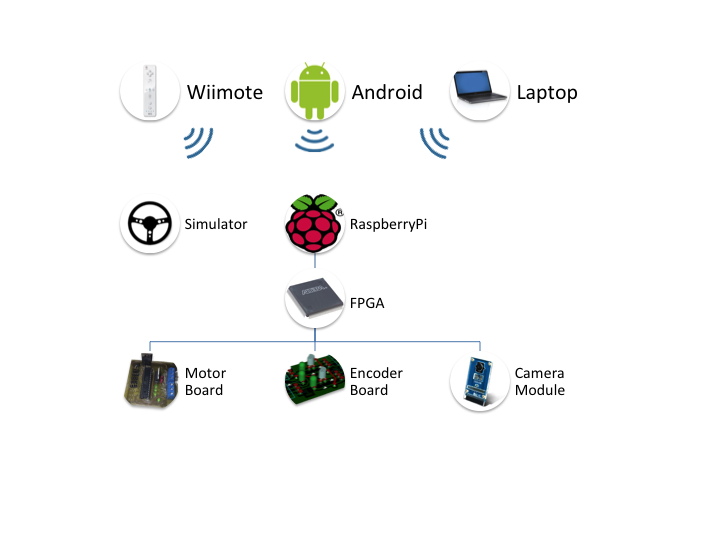
\includegraphics[width=\linewidth]{pic/architecture}
\caption{Architecture overview}
\label{figarchitecture}
\end{center}
\end{figure}

Figure~\ref{figcaroverview} shows, how the above mentioned architecture is realized on the car. All the components are mounted on a wooden plate on top of the car.
\begin{figure}[H]
\begin{center}
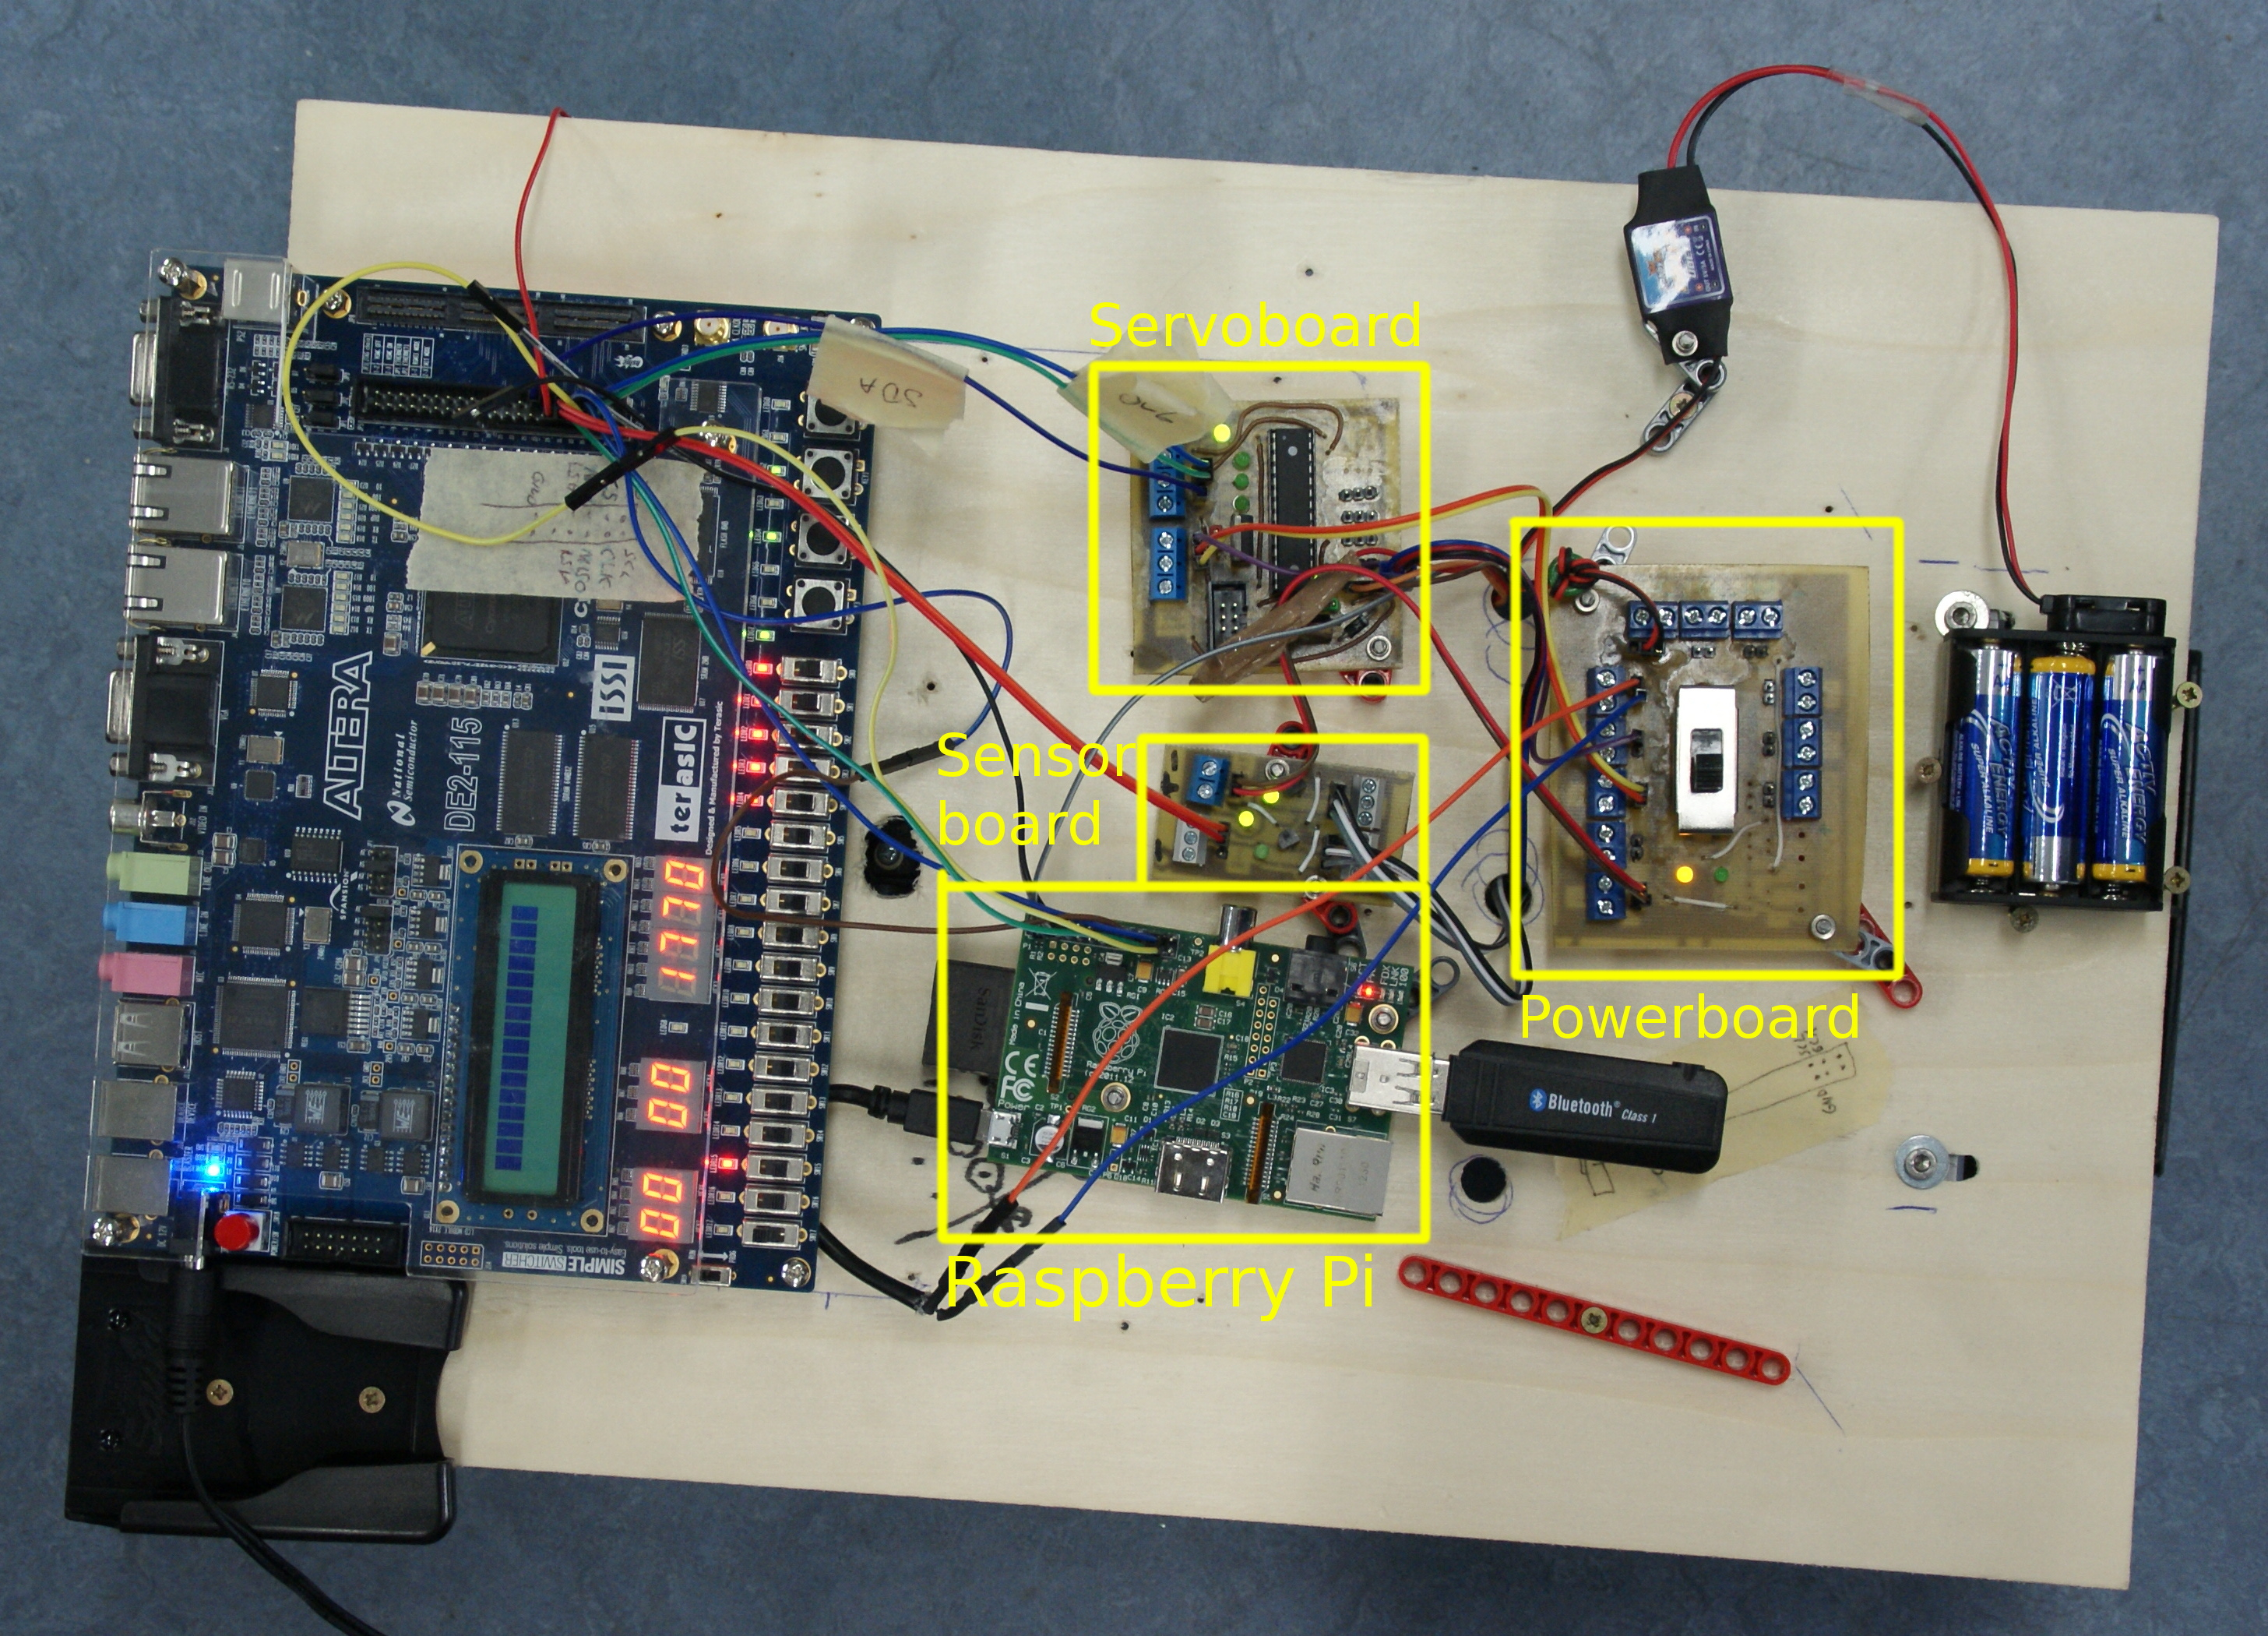
\includegraphics[width=\linewidth]{pic/overview}
\caption{Car overview}
\label{figcaroverview}
\end{center}
\end{figure}

%----------------------------------------------------------------------------------------
\section{Powerboard}
%----------------------------------------------------------------------------------------

Very early in this project, we noticed, that supplying the various boards and modules on the car with power becomes a problem.
This is why we designed a simple board to distribute the power among all components.
The board also has a central on-off switch for all of the needed voltages.
The schematics are very simple an can be seen in Figure \ref{figpowerboardscm}. Figure \ref{figpowerboardr} shows the finished board.

\begin{figure}[H]
\begin{center}
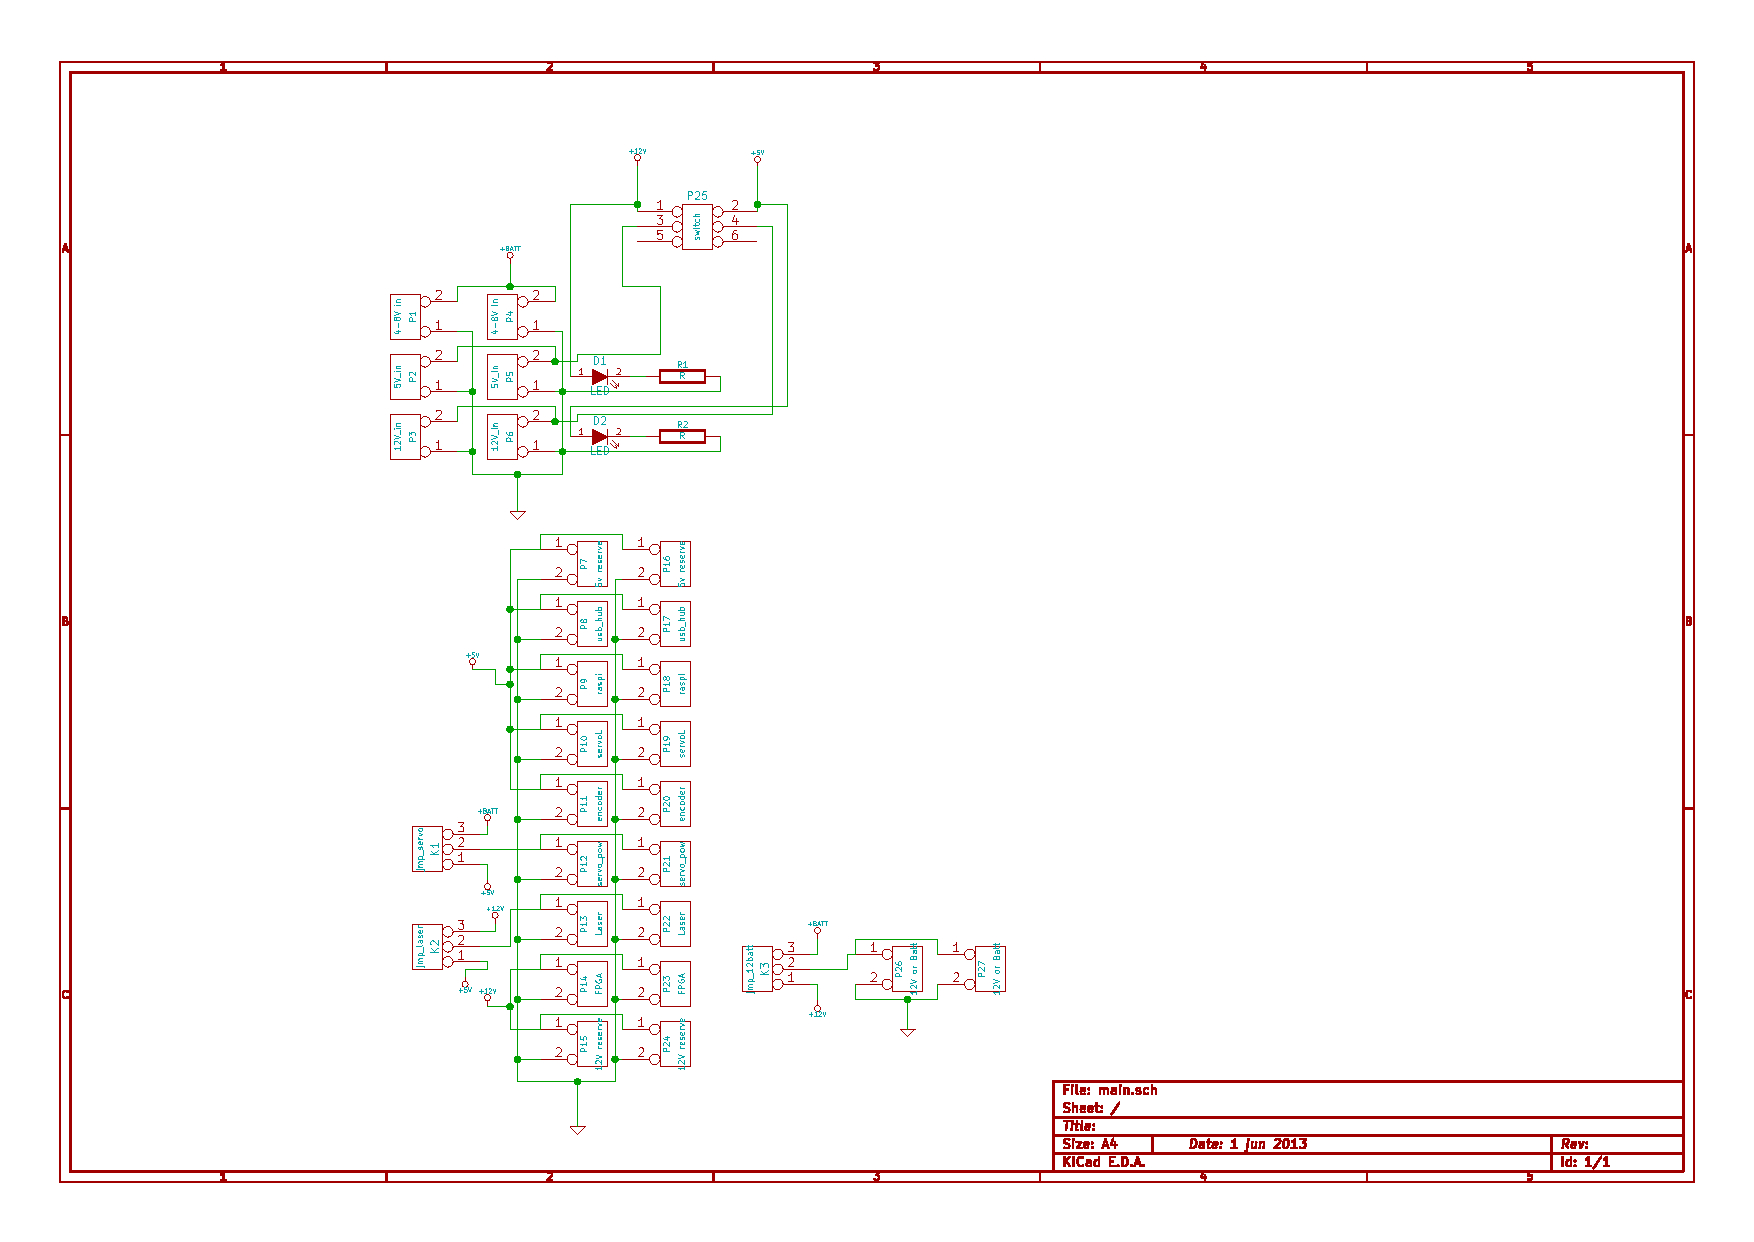
\includegraphics[width=0.7\linewidth]{pic/powerboard}
\caption{Powerboard schematics}
\label{figpowerboardscm}
\end{center}
\end{figure}

\begin{figure}[H]
\begin{center}
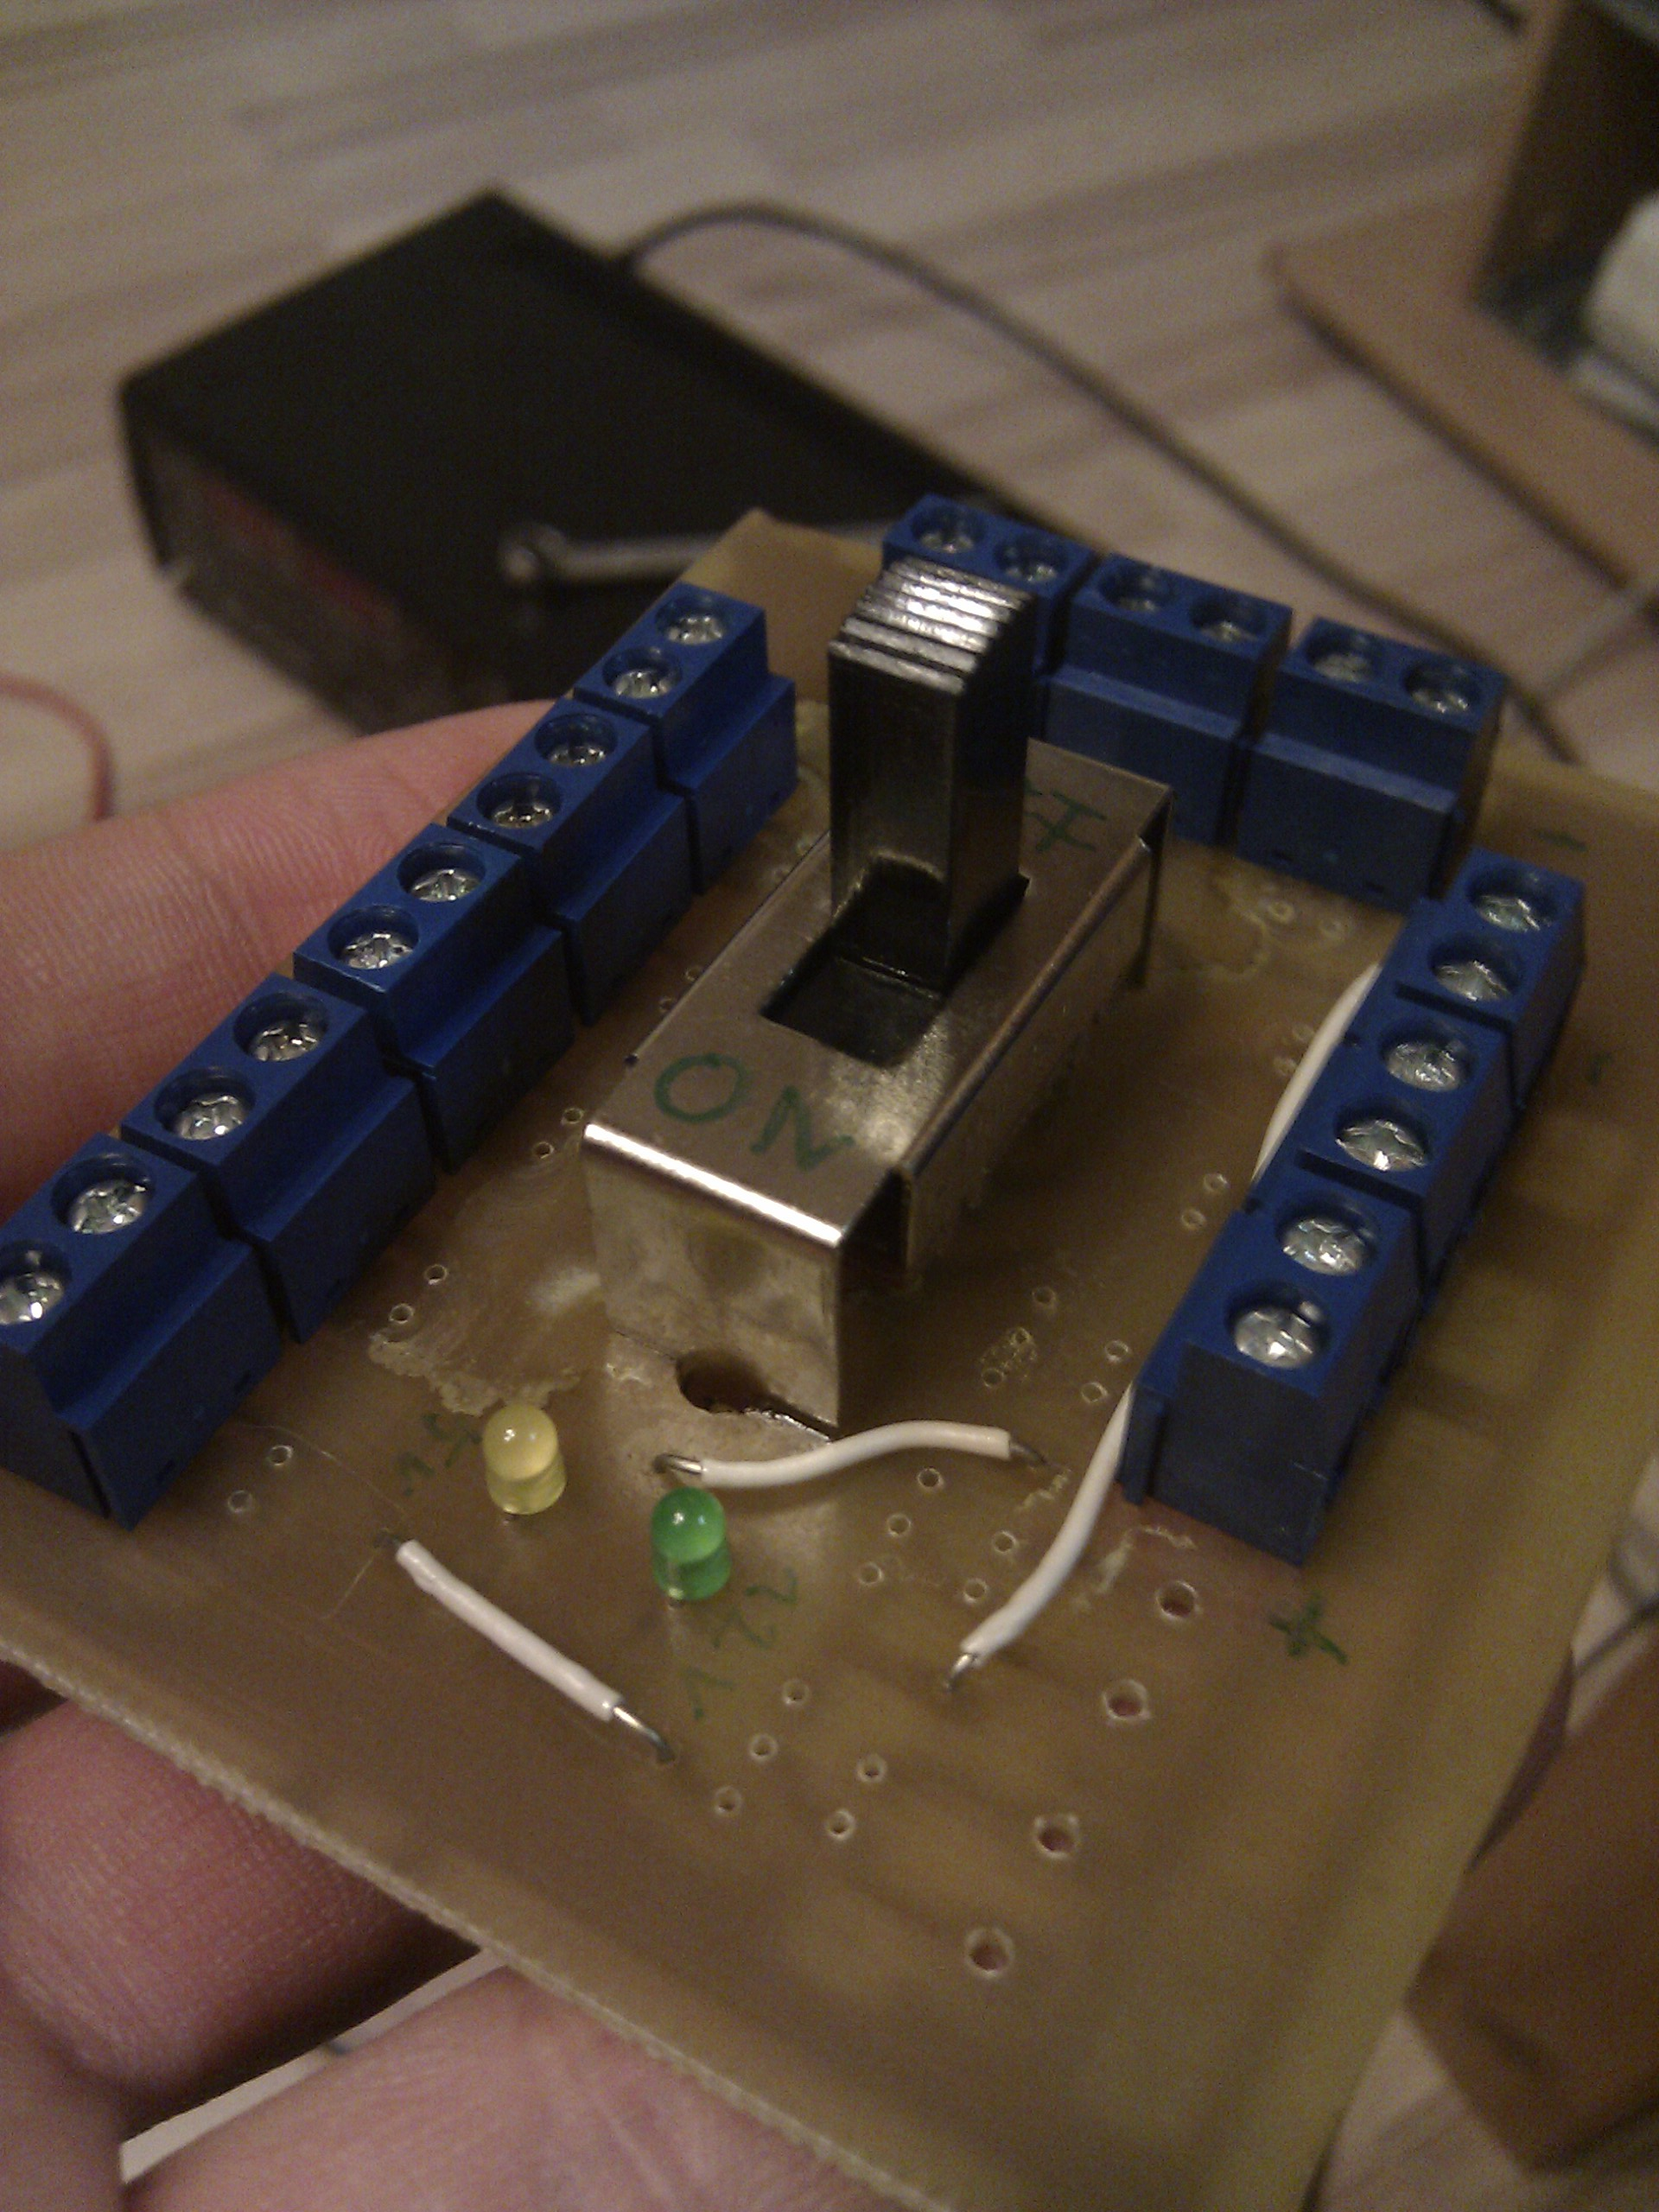
\includegraphics[width=8cm]{pic/powerboardr.jpg}
\caption{Powerboard}
\label{figpowerboardr}
\end{center}
\end{figure}


%----------------------------------------------------------------------------------------
\section{Rotary Encoders} %%TODO: richtige bezeichnung???
%----------------------------------------------------------------------------------------

To measure speed, we built two rotary encoders into the car.
They are based on a simple and cheap light barrier with an included Schmitt trigger and a rotary encoder disc.
A picture and a schematic of the light barriers can be seen in Figure \ref{figls}.
\begin{figure}[H]
\begin{center}
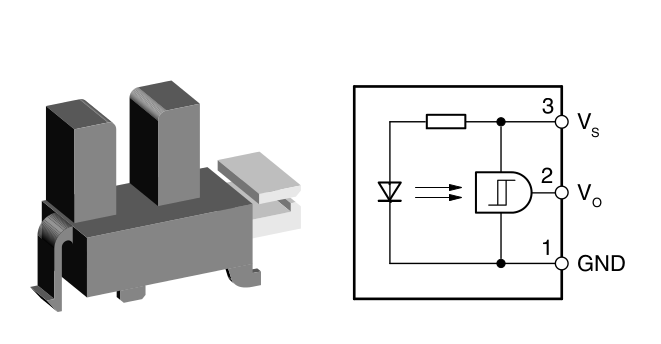
\includegraphics[width=8cm]{pic/ls.png}
\caption{Light barrier}
\label{figls}
\end{center}
\end{figure}

There are four slots in each disc, so that we can measure the speed at the resolution of roughly a quarter of a turn.
The discs are mounted on shafts, which are directly connected to the differentials.
We use two rotary encoders.
One is connected to the front differential and one is connected to the back differential.
The cardan shaft of the initial 4WD car design has been removed to make room for the rotary encoders.
Because of the removed 4WD and the two rotary encoders, it is now possible to measure the speed of the front and the back wheels independently.
This enables us to detect slippage, as only the back wheels are driven by the motor.

Figure \ref{figencmount1} shows the aluminium component that has been manufactured to hold the front rotary encoder shaft in place.
Figures \ref{figencmount2} and \ref{figencmount3} show, how the rotary encoder discs are mounted on the car.

\begin{figure}[H]
  \centering
  \begin{subfigure}[b]{0.3\textwidth}
  \centering
  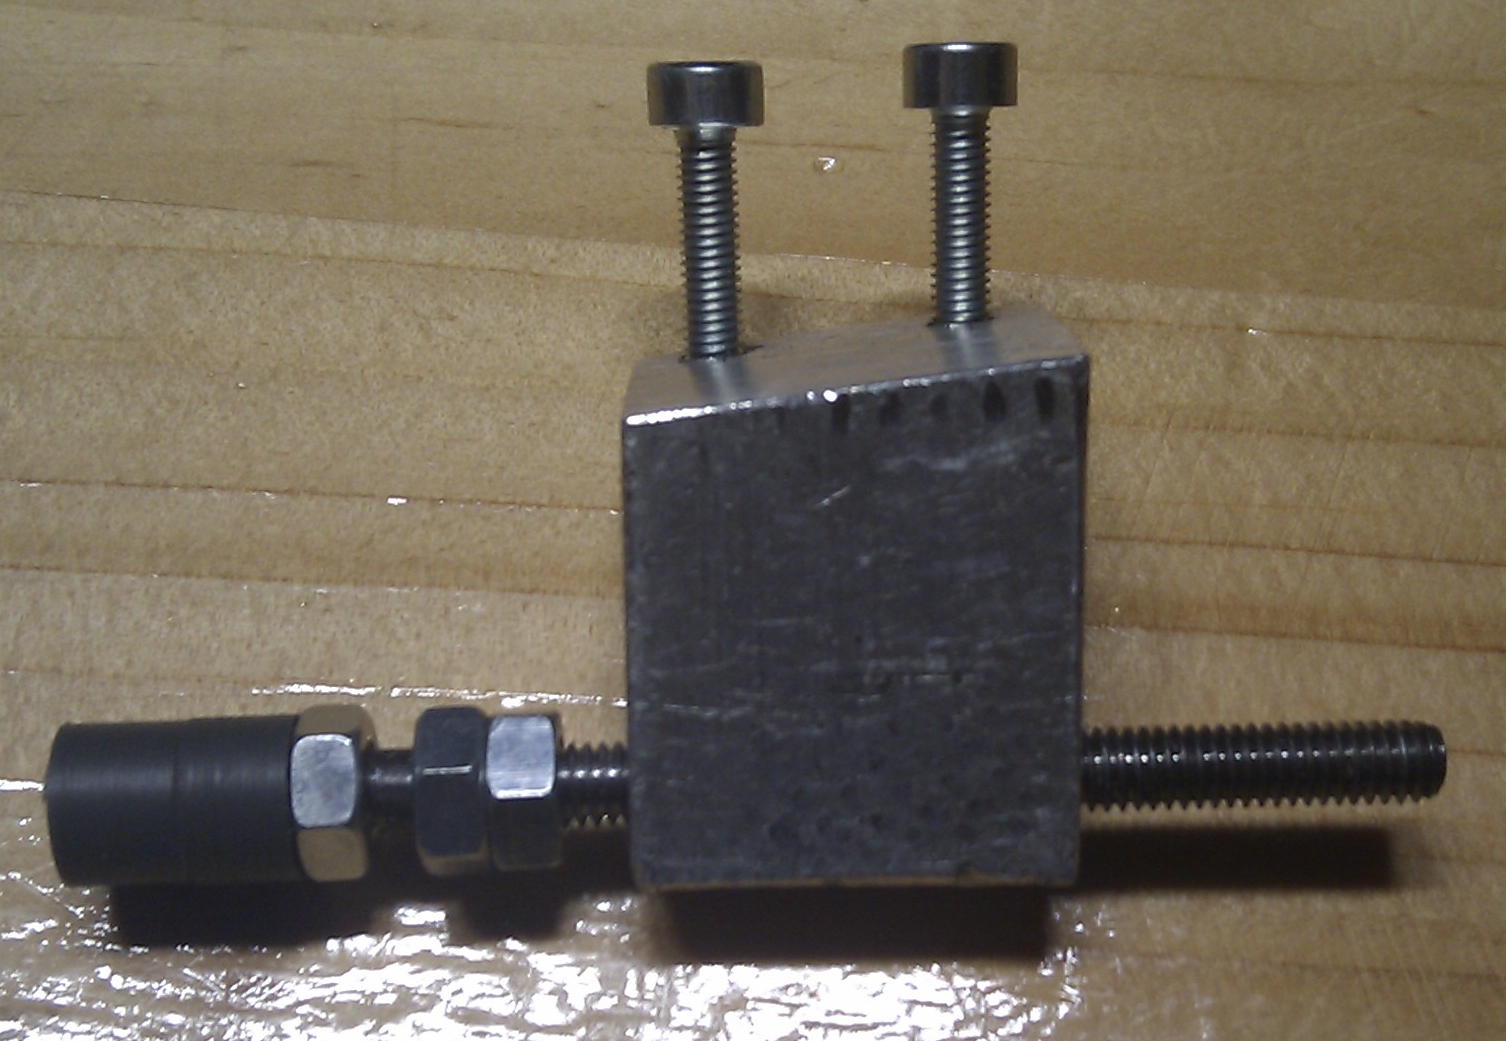
\includegraphics[width=\textwidth]{pic/encoder_mount.png}
  \caption{Custom designed aluminium mounting block}
  \label{figencmount1}
  \end{subfigure}~
  \begin{subfigure}[b]{0.3\textwidth}
  \centering
  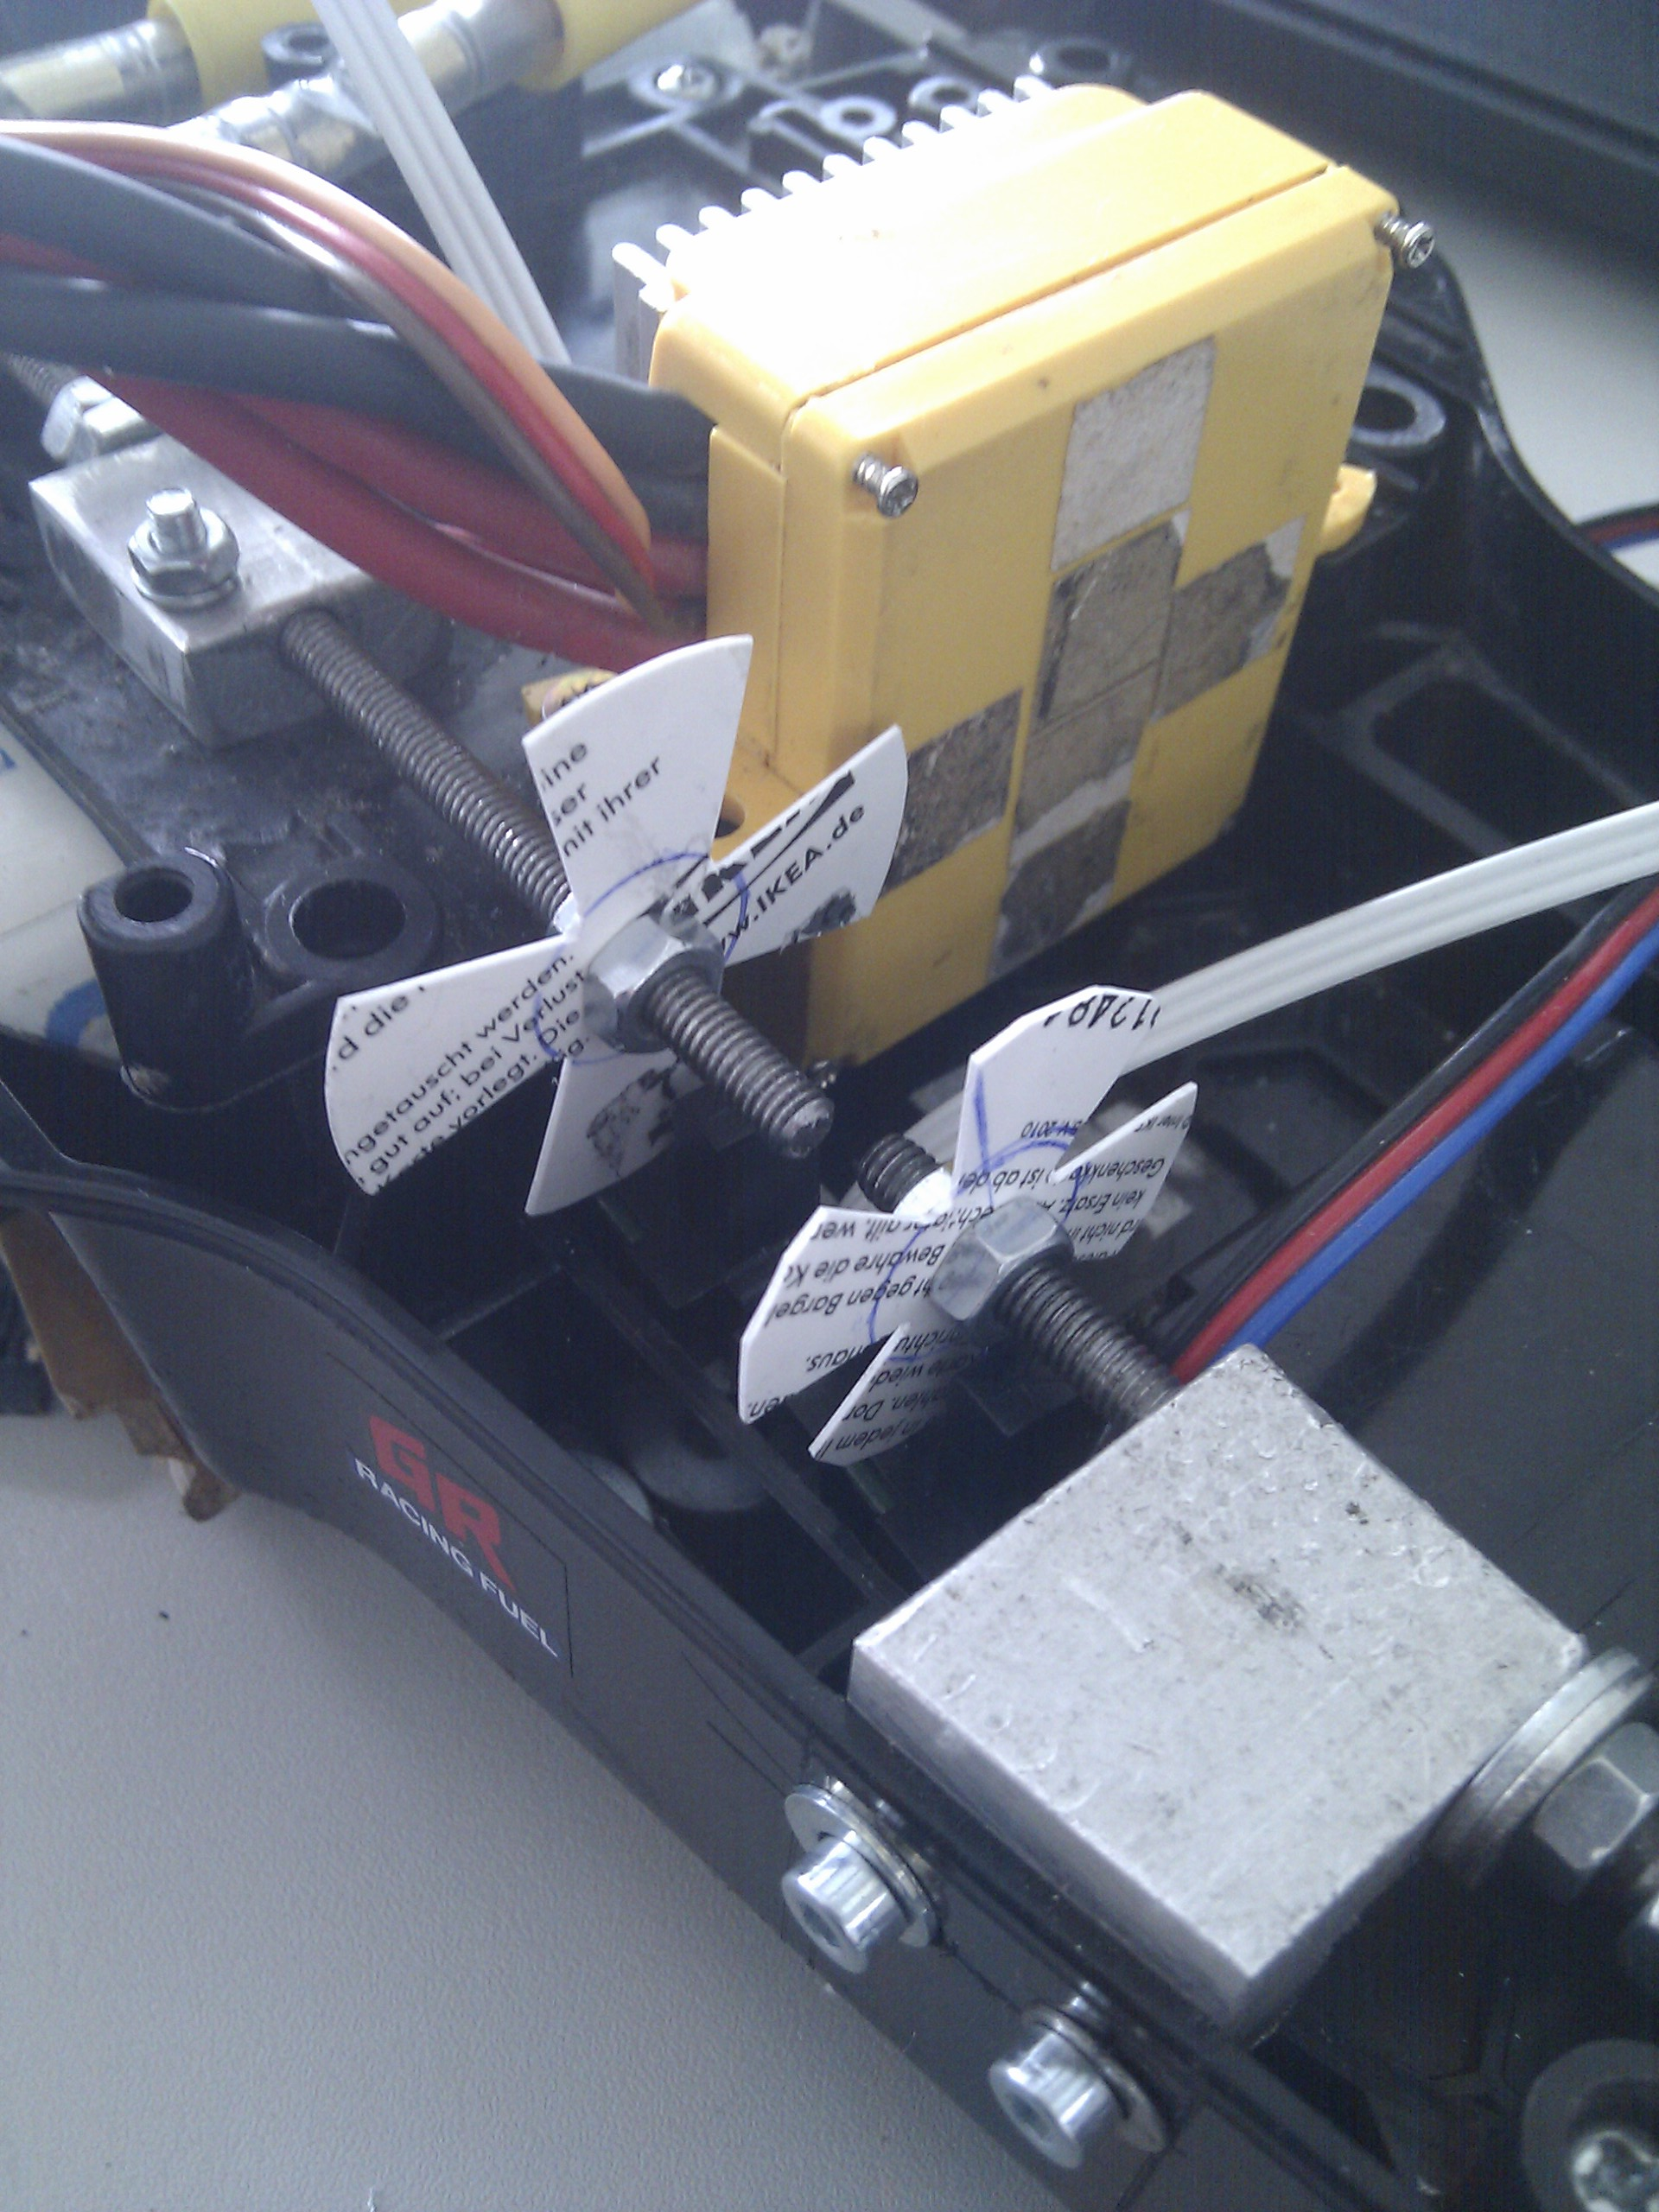
\includegraphics[width=\textwidth]{pic/encoders_scheiben.jpg}
  \caption{Encoders mounted in the car chassis}
  \label{figencmount2}
  \end{subfigure}~
  \begin{subfigure}[b]{0.3\textwidth}
  \centering
  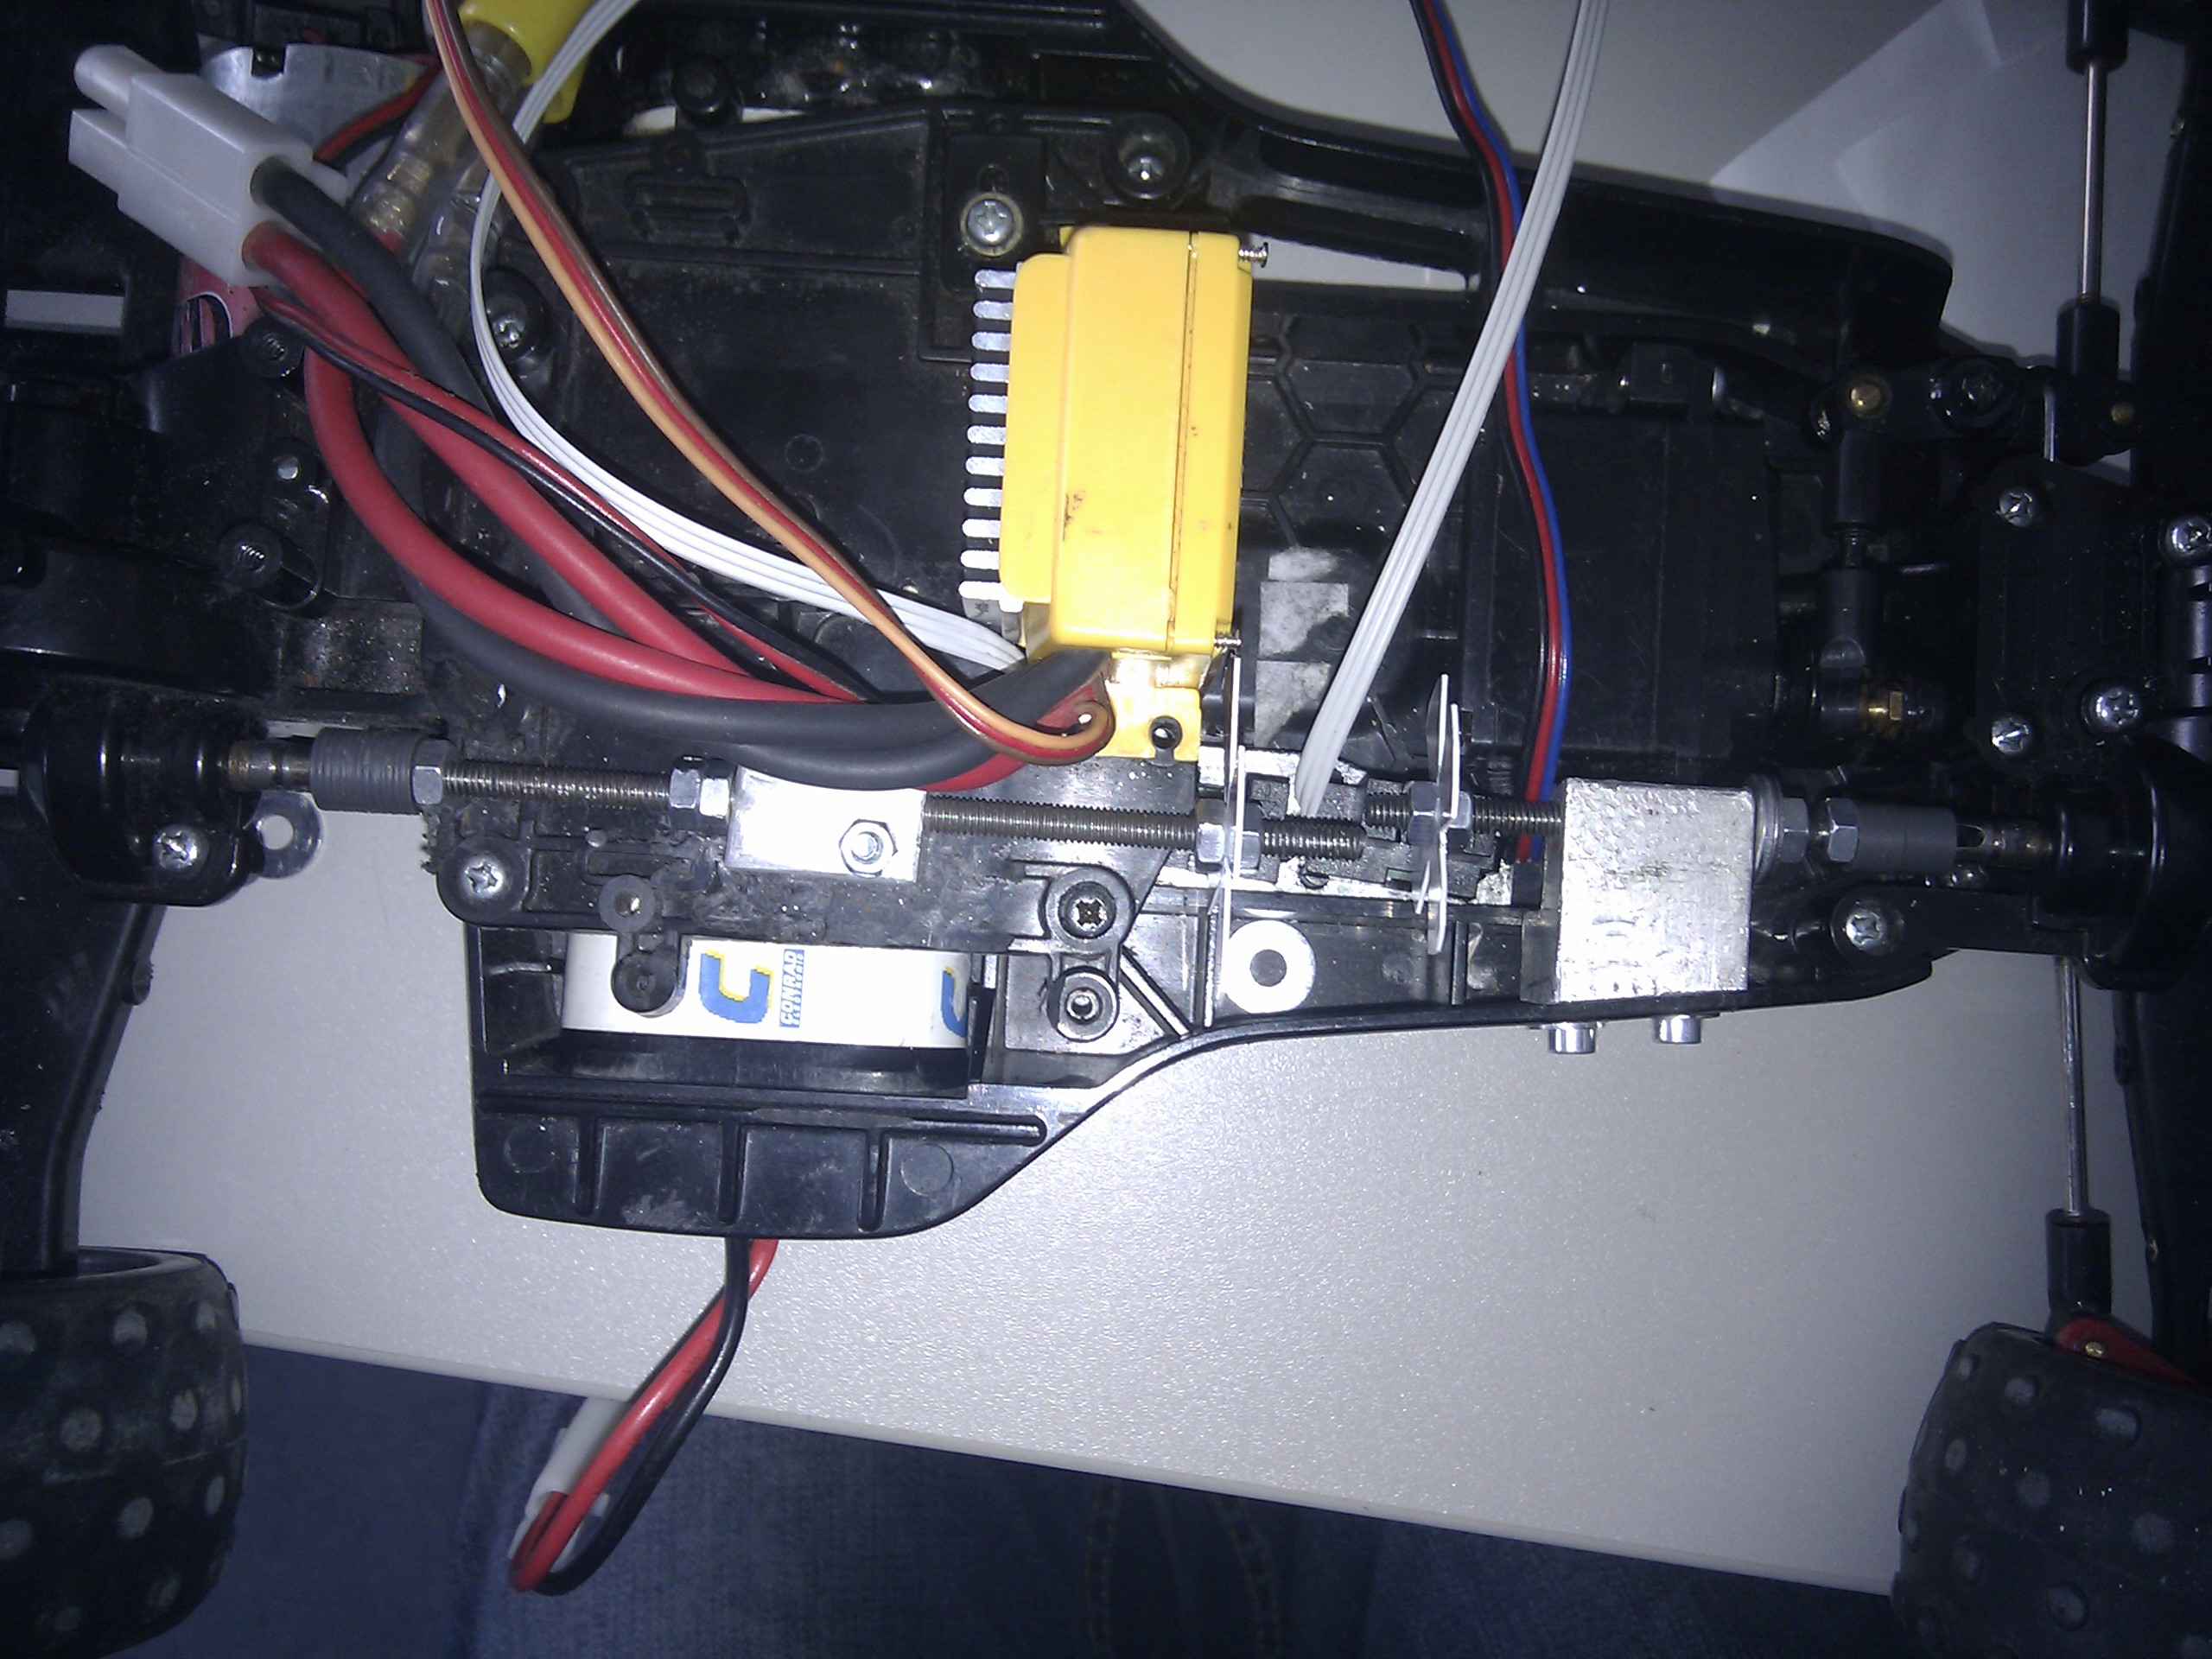
\includegraphics[width=\textwidth]{pic/encoders_top.jpg}
  \caption{Encoders in the car}
  \label{figencmount3}
  \end{subfigure}
  \caption{Encoder mounting}
  \label{figenc}
\end{figure}


To connect the light barriers to the FPGA, we built a Sensorboard. It has the task to supply the light barriers with power and to convert the output voltage of the light barriers to the right level.
There are also two LEDs on the board, that show the current state of the light barriers.
This made it easier to debug the light barriers when moving the rotary encoder discs into position.
The schematics of the Sensorboard can be seen in Figure \ref{figsensorboardscm}. The board layout and a 3D rendering can be seen in Figures \ref{figsensorboardbrd} and \ref{figsensorboard3d}.

\begin{figure}[H]
  \centering
  \begin{subfigure}[b]{0.5\textwidth}
  \centering
  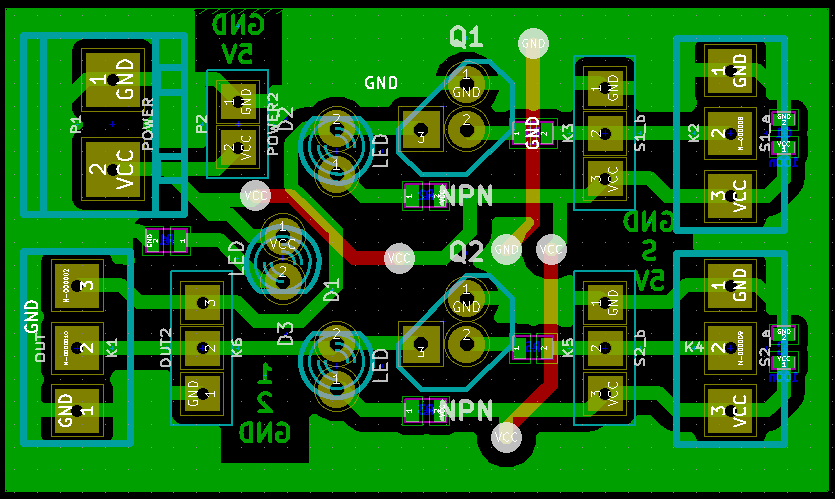
\includegraphics[width=\textwidth]{pic/sensorboardbrd.png}
  \caption{Layout}
  \label{figsensorboardbrd}
  \end{subfigure}~
  \begin{subfigure}[b]{0.5\textwidth}
  \centering
  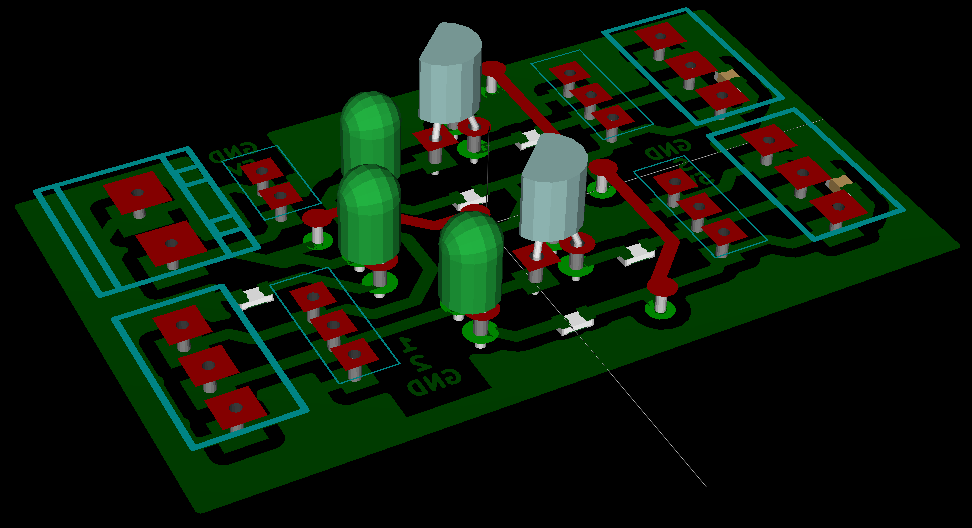
\includegraphics[width=\textwidth]{pic/sensorboard3d.png}
  \caption{3D render}
  \label{figsensorboard3d}
  \end{subfigure}
  \caption{Sensorboard}
  \label{figsensorboard}
\end{figure}


\begin{figure}[htb]
\begin{center}
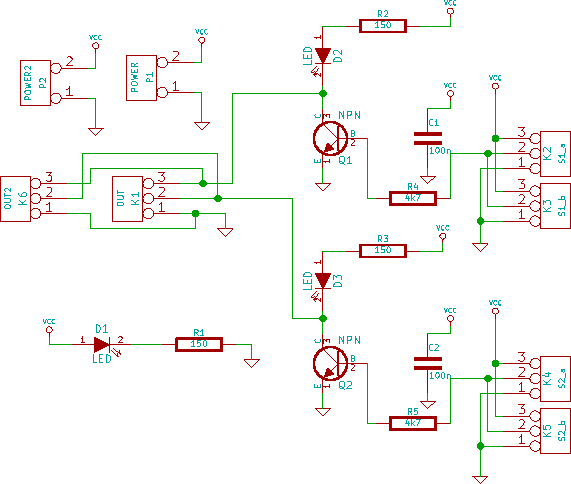
\includegraphics[width=0.7\textwidth]{pic/sensorboard}
\caption{Sensorboard schematics}
\label{figsensorboardscm}
\end{center}
\end{figure}
%----------------------------------------------------------------------------------------
\section{Servo controller board}
%----------------------------------------------------------------------------------------
%%TODO: bildchen

%%TODO: servo-parameter (0-4000-8000)
\subsection{Schematics}

\begin{figure}[H]
\begin{center}
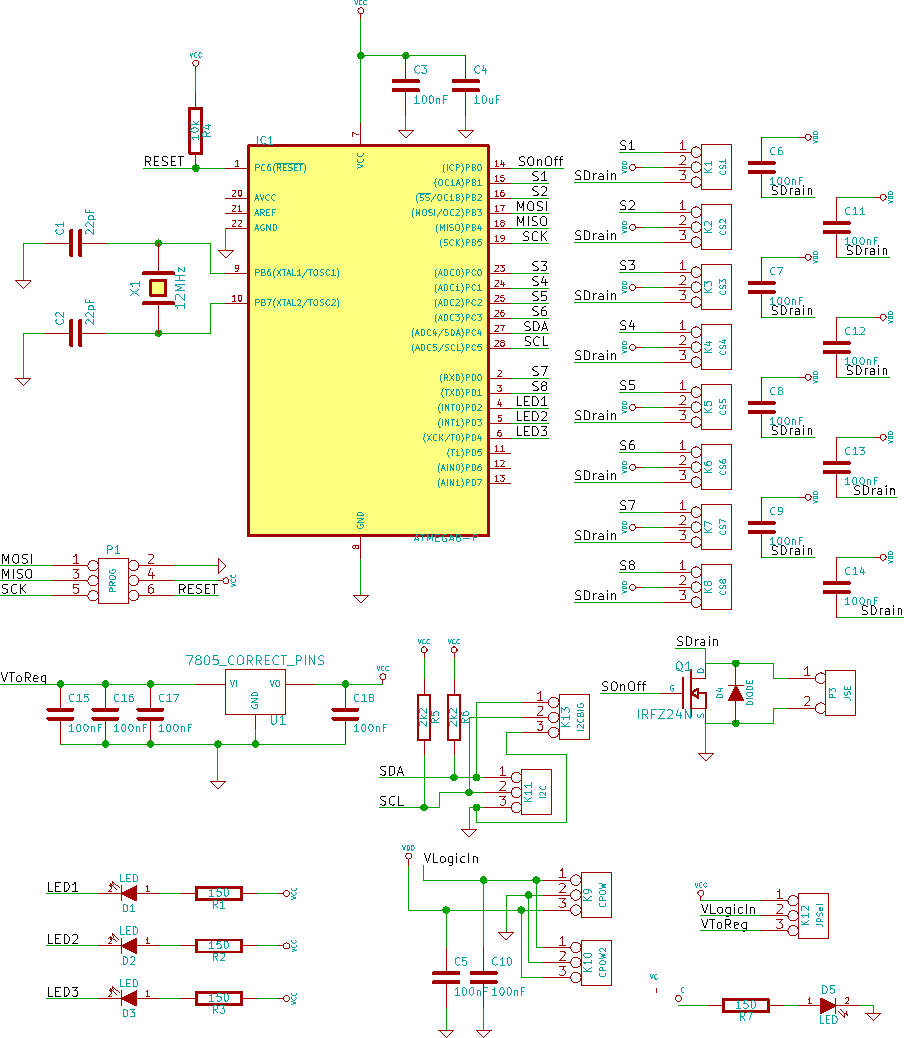
\includegraphics[width=\linewidth]{pic/servoboard}
\caption{Servoboard schematics}
\label{figservoboardscm}
\end{center}
\end{figure}

\subsection{Board}
After the schematics have been created, the PCB board layout was designed.
The components are placed on the board and connected with the corresponding copper tracks.
This process is also called routing.
Routing wasn't a big problem, as we had enough room on the board.
Almost all tracks fitted on one layer and only a few vias and additional floating wires were needed.
This made the PCB manufacturing process easier, as only a one-sided PCB could be used.
Figure \ref{figservoboardbrd} shows the finished board layout, Figure \ref{figservoboard3d} shows a 3D rendering of the Servoboard and the finished board can be seen in Figure \ref{figservoboardr}.

\begin{figure}[H]
  \centering
  \begin{subfigure}[b]{0.3\textwidth}
    \centering
    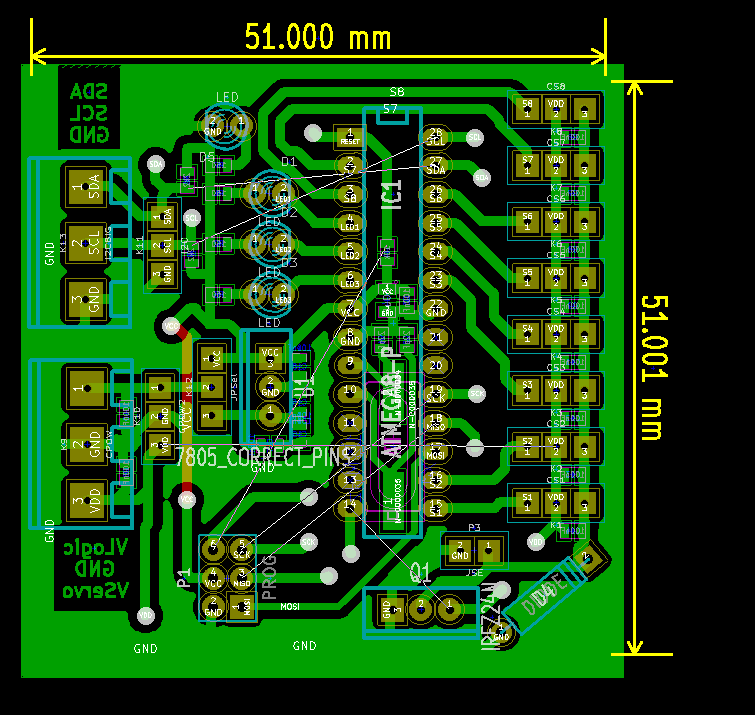
\includegraphics[width=\textwidth]{pic/servoboardbrd.png}
    \caption{Layout}
		\label{figservoboardbrd}
  \end{subfigure}~
  \begin{subfigure}[b]{0.3\textwidth}
    \centering
    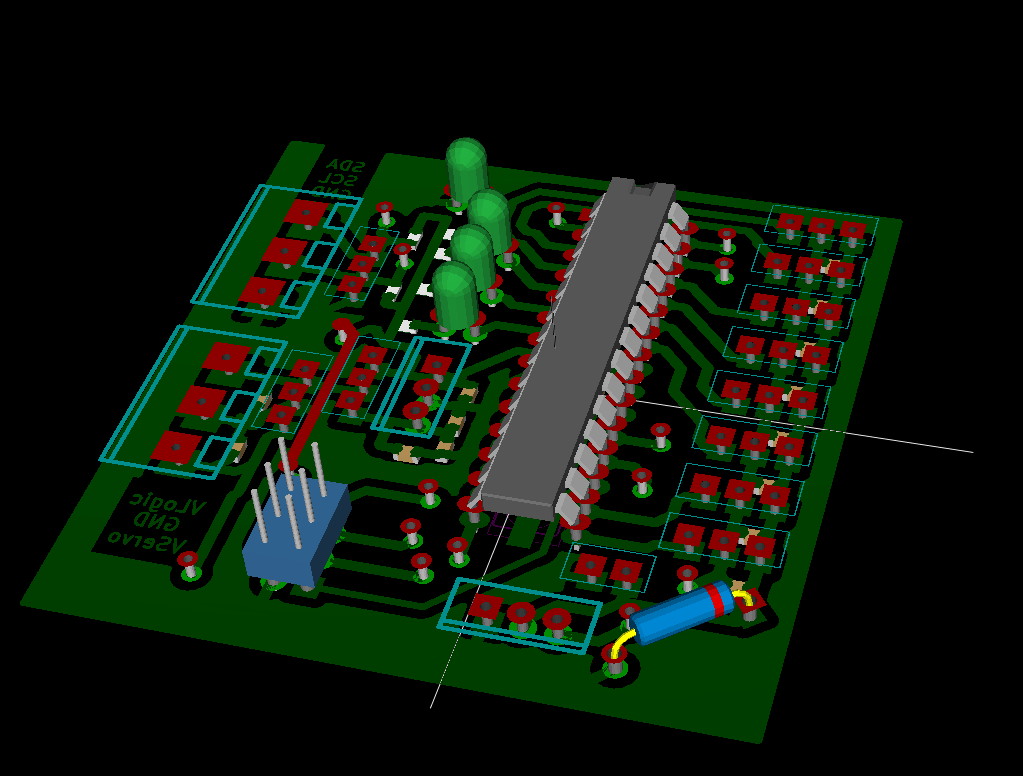
\includegraphics[width=\textwidth]{pic/servoboard3d.png}
    \caption{3D rendering}
		\label{figservoboard3d}
  \end{subfigure}~
  \begin{subfigure}[b]{0.3\textwidth}
    \centering
    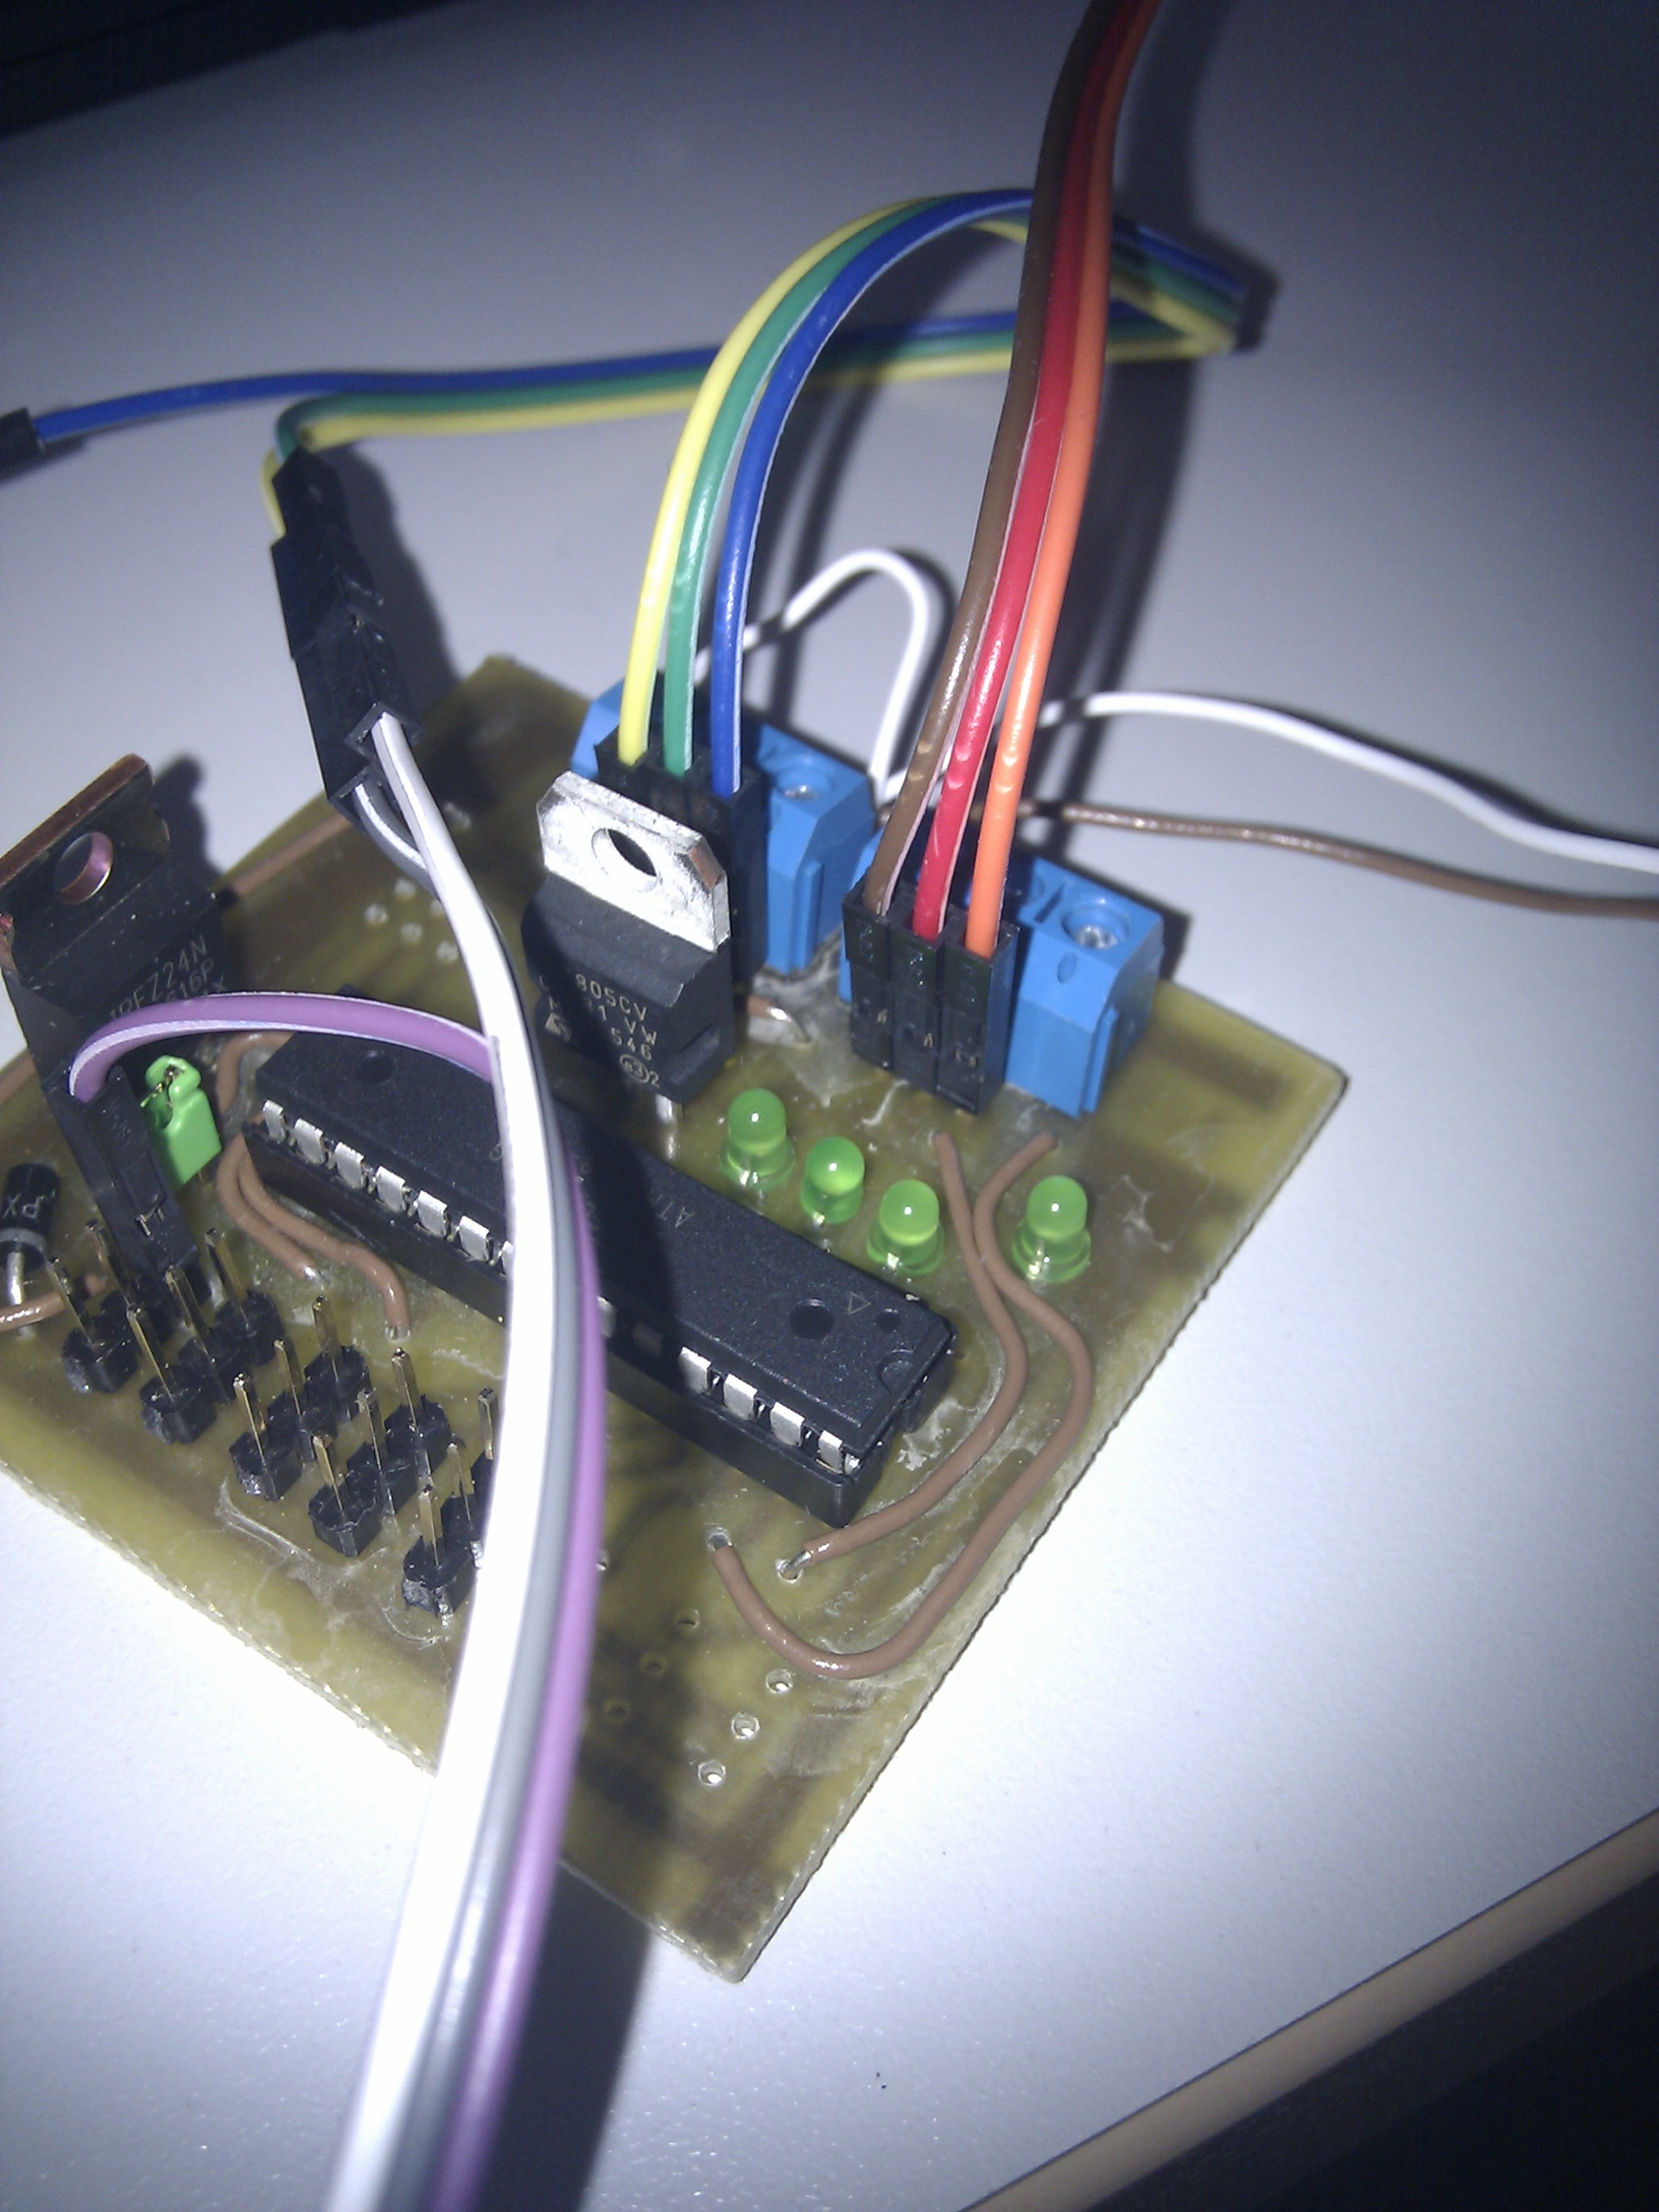
\includegraphics[width=\textwidth]{pic/servoboardr.jpg}
    \caption{Final assembly}
		\label{figservoboardr}
  \end{subfigure}
  \caption{Servoboard}
\end{figure}
\subsection{Communication protocol}
The Servoboard is connected via the I2C or two-wire interface to a command unit.
The command unit can either be the FPGA or the RaspberryPi.


The I2C protocol is not implemented in software, but the hardware I2C capabilities of the AVR Atmega8 microcontroller are used.
This gives us faster response time and less overhead.
It also unburdens the AVR CPU, as only one hardware interrupt is needed, each time a complete byte is received via I2C.
Implementing I2C via software would have required many timer interrupts and might have turned out less stable.


We implemented our own communication protocol on top of I2C.
In the microcontroller's firmware, we used a simple state machine to realize this.

The communication protocol looks as follows:
The Master first sends a preamble (0xff), which is used to synchronize both communication partners.
This is necessary, because loosing packets or receiving corrupted data can lead to a situation, where the receiving unit ends up in an undefined or faulty state.
Therefore, it might be that the communication gets stuck.

By sending a preamble, that cannot be part of the normal communication, this problem is solved: Every time the microcontroller receives a preamble-byte, the communication state machine goes back to its initial state, no matter what the current state is.
This way, if a transmission error occurs, only the current command is lost, but further communication will still be possible.


Nevertheless, our communication protocol makes it possible to transmit 0xff inside a command using the following method:
If values greater or equal than 254 are sent, they are split into two bytes.
The first byte is 254 and the next one is the difference to the desired number.
On the receiver's side, both values are then combined and their sum determines the actual number. 
For example if 255 needs to be sent, the two bytes 254 and 1 are sent.

\subsection{Firmware}

\section{RaspberryPi}
The RaspberryPi is used for highlevel communication.
It is connected to a wifi module via USB and opens up an access point.
The RasPi is also equipped with a bluetooth module to communicate with a Wiimote controller.

\subsection{Software}
On the RaspberryPi, there runs the raspi.exe program, which can be found in the \textit{raspi} folder.
It will start up a TCP/IP server and listen for a Wiimote controller via bluetooth.
Over those interfaces, it will accept highlevel commands to control the car.
Note that only one device is able to control the car at a time.
There is a handover mechanism implemented in the \textit{raspi.exe} program: If a device sends a \textit{getperm}-command, it will take over the control and commands from other currently connected devices are ignored.


The configuration of the raspi.exe program is done via the file \textit{config.h}:
SERVO\_M defines, to which module the RasPi software will send its commands. The possible values are:
\begin{itemize}
\item{SERVO\_SIM}
\item{SERVO\_BOARD}
\item{SERVO\_FPGA}
\end{itemize}

If SERVO\_SIM is set, \textit{raspi.exe} will send the commands to a simulation program via TCP/IP.
The IP and TCP port of the simulation program can also be configured in the \textit{config.h} file.
The \textit{raspi.exe} will send its commands directly to the Servoboard via I2C, if SERVO\_M is set to SERVO\_BOARD.
The last option SERVO\_FPGA causes \textit{raspi.exe} to talk to the FPGA board via SPI.

If a Wiimote controller should be used to control the car, WII\_ENABLED must be set to 1 in the \textit{config.h} file.
Communication via TCP/IP is always enabled.

Settings, which are more specific to one communication unit, can be configured in \textit{servoboard.h, servosim.h} or \textit{fpga\_spi.h} respectively. Those files contain the parameters for the I2C or SPI specific communication, such as addresses, speeds or the paths to the chardevs.

\subsection{TCP communication protocol}
The \textit{raspi.exe} TCP server accepts the following commands:
\begin{description}
\item[servo set $<$channel$>$ $<$valve$>$] Sets the servo which is connected on PIN $<$channel$>$ to the corresponding value. $<$channel$>$ must be an integer between 0 and 7. $<$value$>$ is also an integer. It can have values from 0 to 8000, where 4000 would mean the zero position.
\item[servo led $<$onoff$>$ $<$mask$>$] Sets the LEDs on the Servoboard. $<$onoff$>$ decides, whether the LEDs should be switched on(1) or off(0). The three LSBs of $<$mask$>$ decide, which LEDs should be switched. Only LEDs, where the bit in the mask is set to 1 will be switched on or off. For example, if one wants to enable the first and the third LED, one would send the command "servo led 1 5". Note that most of the LEDs are by default also used by the Servoboard firmware to signal various events. Once a LED has been manually set to a certain state by setting a bit to one in $<$mask$>$, this LED will not be used by the firmware anymore.
\item[servo getperm] This command initiates an control handover to the device, which is sending this command. From now on, \textit{raspi.exe} will only accept control commands from this device. All other currently connected devices will be ignored.
\item[speedv set $<$speed$>$ $<$steering$>$] This is a highlevel command, which is only accepted, if the RasPi is connected to the FPGA. $<$speed$>$ and $<$steering$>$ are both double values.
\end{description}

\subsection{Remote control devices}
The car can be controlled by any device that supports TCP/IP over wifi.
So for example it is possible to control the car via a notebook that is connected to the car's wifi access point.
To demonstrate the remote control capabilities of the car's software, we implemented an Android client. Screenshots of this client can be seen in Figures \ref{figand1} and \ref{figand2}.
\begin{figure}[H]
  \centering
  \begin{subfigure}[b]{0.7\textwidth}
    \centering
    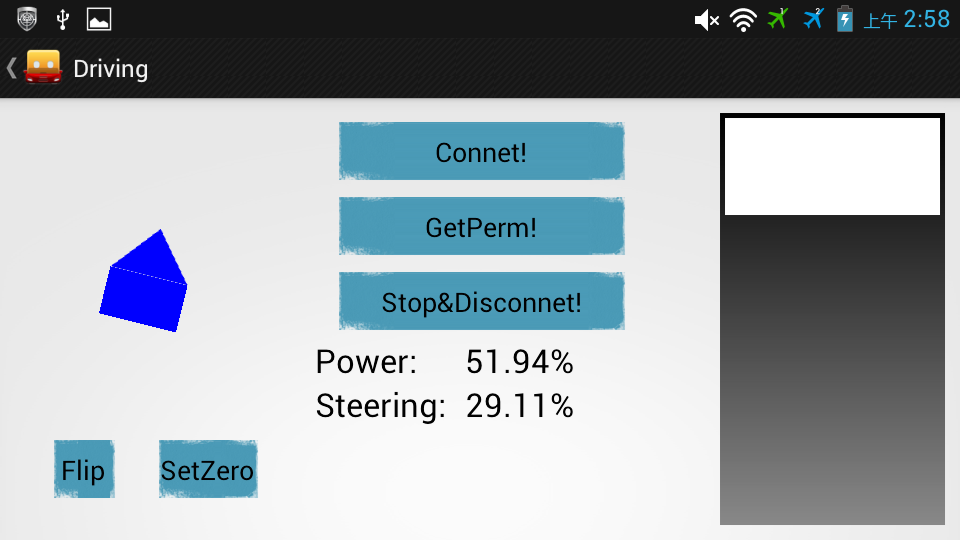
\includegraphics[width=\textwidth]{pic/figand1.png}
    \caption{Control}
		\label{figand1}
  \end{subfigure}~
  \begin{subfigure}[b]{0.3\textwidth}
    \centering
    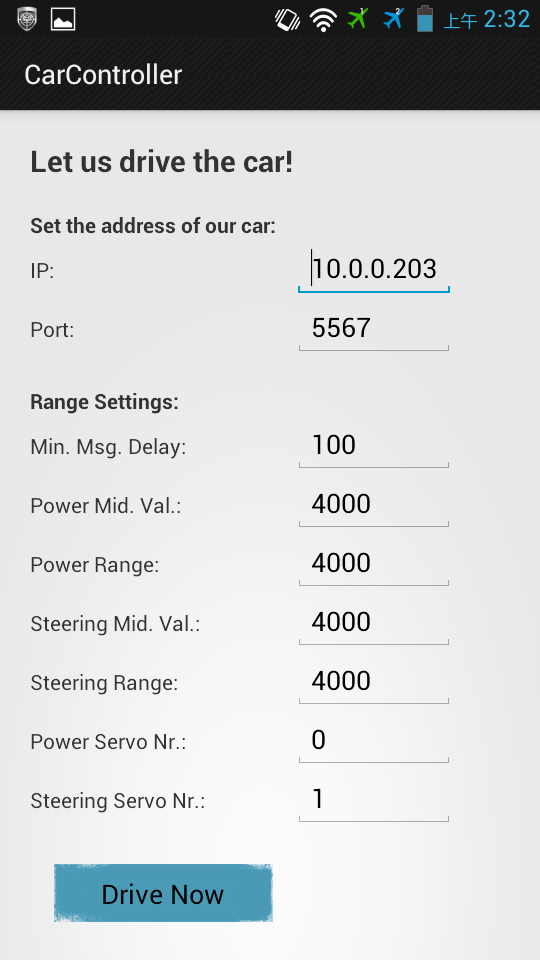
\includegraphics[width=\textwidth]{pic/figand2.png}
    \caption{Settings}
		\label{figand2}
  \end{subfigure}
  \caption{Android remote control client}
\end{figure}

Another option is to use a Wiimote remote to control the car. If the WII\_ENABLED option is set in the \textit{raspi.exe} configuration, the RaspberryPi software will periodically try to connect to a Wiimote controller.
Button 1 and 2 need to be pressed simultaneously on the Wiimote controller to enter the discovery procedure.
Once the Wiimote remote is connected to the RaspberryPi, the car can be controlled.
The Wiimote has the following key assignment:
\begin{description}
\item[+] Accquire control over the car (initiate handover mechanism)
\item[-] Enable/disable traction control system (only active in speed control mode)
\item[Home] Switch between speed control mode and acceleration mode
\item[A] Switch acceleration mode from \textit{button} to \textit{tilt} and vice-versa
\item[1] Accelerate slowly
\item[1+2] Accelerate
\item[2] Accelerate fast
\item[left] Accelerate backwards
\item[tilt left/right] Steer left/right
\item[tilt forward/backward] Accelerate forward/backward
\end{description}


%----------------------------------------------------------------------------------------
\section{FPGA}
%----------------------------------------------------------------------------------------

\subsection{Overview}

\begin{figure}[H]
\begin{center}
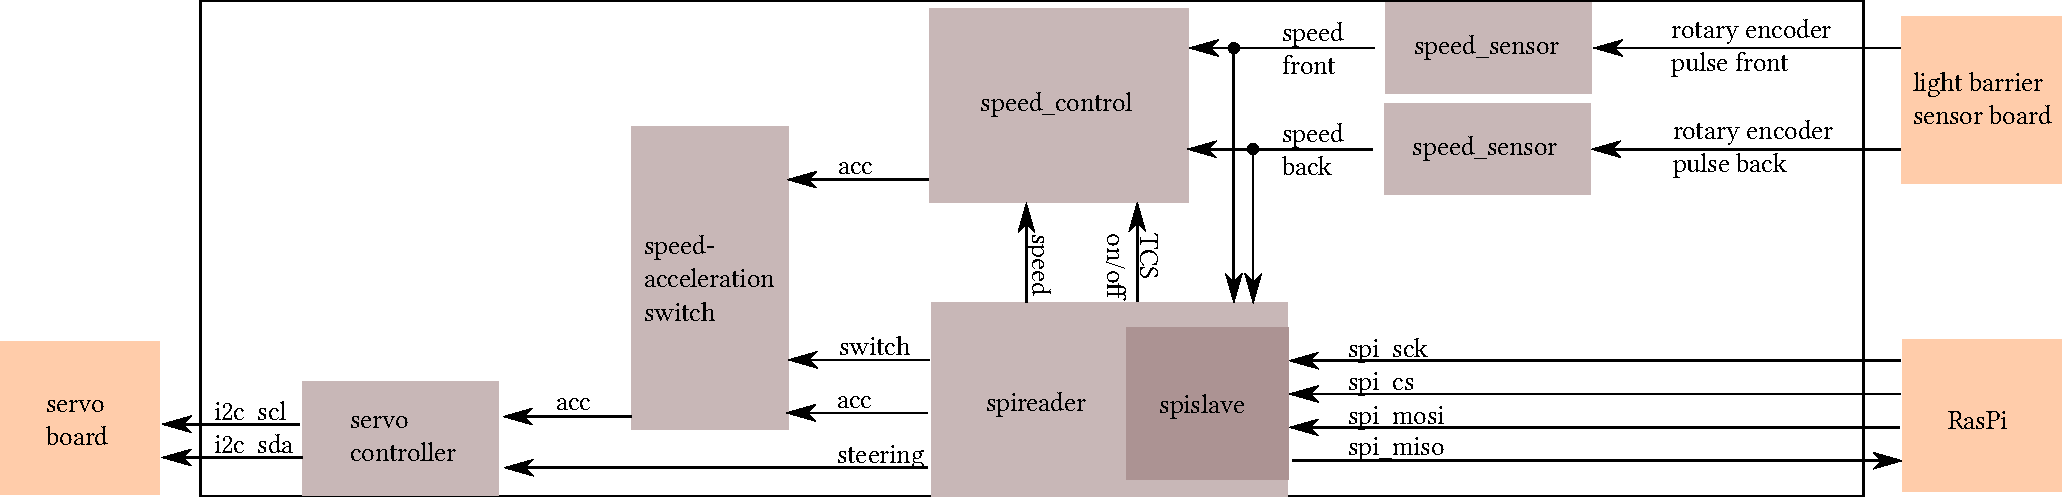
\includegraphics[width=\linewidth]{pic/fpga}
\caption{FPGA overview}
\label{figfpga}
\end{center}
\end{figure}



\subsection{Speed control}
We designed the VHDL \emph{speed\_control} architecture to convert a desired speed received from the upper level logic into a supply current for the car's engine. To achieve best possible accuracy the meassured speed on each axis, as well as the desired speed are processed, depending on the operating mode. In the following the two operating modes \emph{Simple speed regulation} and \emph{traction control} are described and evaluated in detail.
\subsubsection{Simple speed regulator}
In this mode the \emph{speed\_control} tries to reach the desired speed $v_{dest}$ by directly regulating the rear wheel to the desired speed, assuming, that the speed of this wheel is the speed of the car.\\
The speed segulating is done by implementing an PI-Regulator. The regulator interval is $\frac{1}{10}s$. Every timestep the difference between desired and current wheelsped is calculated:
$$\Delta = v_{dest} - v_{rear}$$
The calculated difference is then summed up to implement the integral part of the regulator:
$$\Delta_{sum} += \Delta$$
The output power to the engine calculates as follows:
$$power = c_P \cdot \Delta + c_I \cdot \Delta_{sum}$$
Thereby $c_P$ and $c_I$ are constant parameters and need to be tuned to acheive optimum behaviour. $c_P$ configures the proportional part of the regulator. the higher the value, the faster the response of the regulator. But too high values make the system unstable. The $c_I$ is responsible for the integral part of the regulator, which stabilizes the regulator by allowing it to converge to a 
\begin{figure}[H]
  \centering
  \begin{subfigure}[b]{0.5\textwidth}
    \centering
    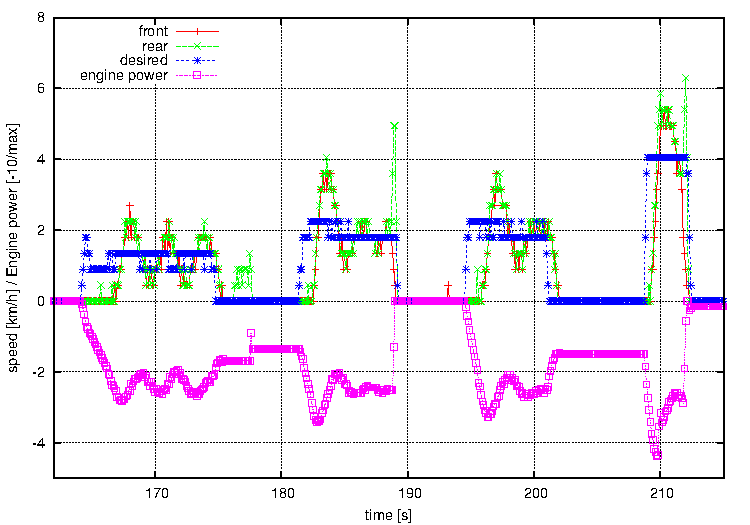
\includegraphics[width=\textwidth]{pic/plot_slow/plot.pdf}
    \caption{Multiple runs}
		\label{figand1}
  \end{subfigure}~
  \begin{subfigure}[b]{0.5\textwidth}
    \centering
    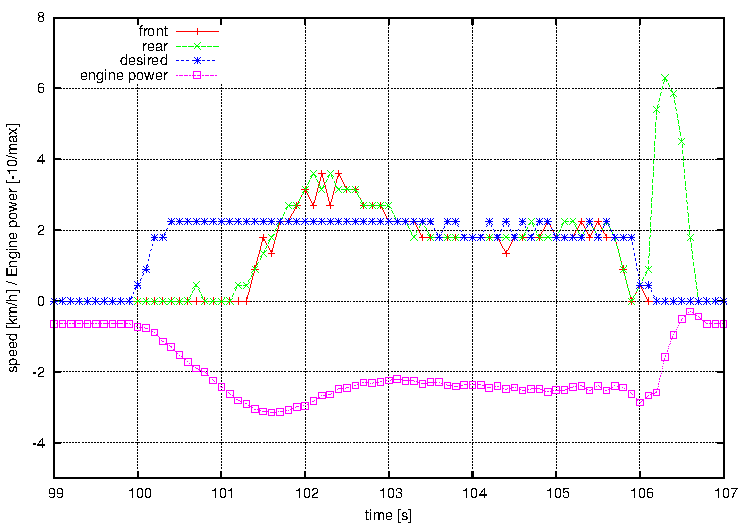
\includegraphics[width=\textwidth]{pic/plot_slow2/plot.pdf}
    \caption{One run at a desired speed of $2 \frac{km}{h}$}
		\label{figand2}
  \end{subfigure}
  \caption{Regulating to the desired speed at the low end of the possible speeds. The Peaks of the rear wheel speed are caused by lifting the car from the ground after the test.}
\end{figure}

\subsubsection{Traction control}
\begin{figure}[H]
  \centering
  \begin{subfigure}[b]{0.5\textwidth}
    \centering
    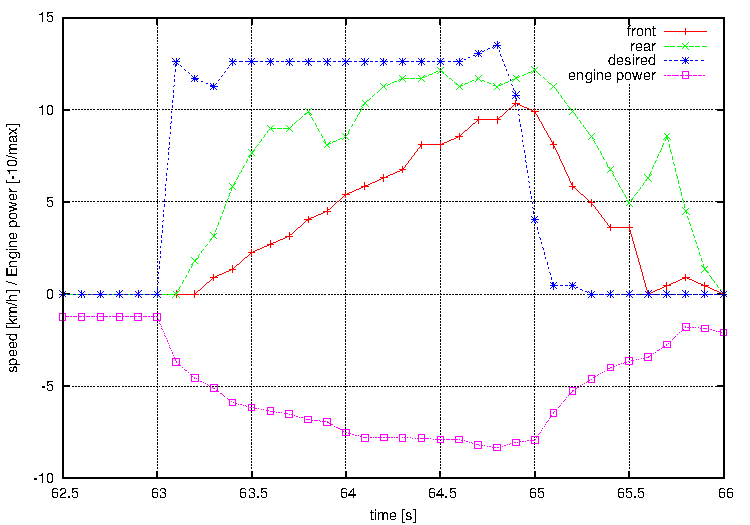
\includegraphics[width=\textwidth]{pic/plot_burnout/plot.pdf}
    \caption{Traction control turned off. Car was stopped by setting the desired speed to zero.}
		\label{figand1}
  \end{subfigure}~
  \begin{subfigure}[b]{0.5\textwidth}
    \centering
    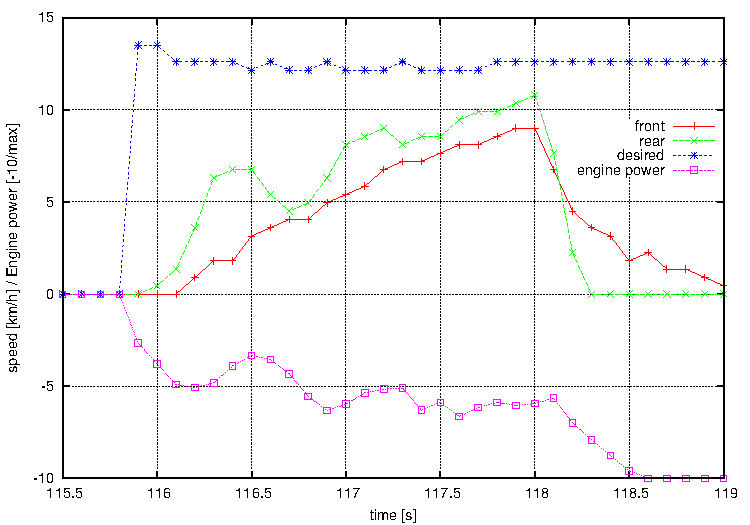
\includegraphics[width=\textwidth]{pic/plot_burnout_asr/plot.pdf}
    \caption{Traction control turned on. Car was stopped by hand, while desired speed was still at $13 \frac{km}{h}$.}
		\label{figand2}
  \end{subfigure}
  \caption{Acceleration phase during burnout test}
\end{figure}
%----------------------------------------------------------------------------------------
\section{Simulator}
%----------------------------------------------------------------------------------------


After staring up the simulator, the car can be driven via the arrow keys. When pressing \textit{C}, one can delegate the control to the built-in TCP server. The current state is shown in the upper left corner.
When the control mode is switched to \textit{TCP}, the simulator accepts commands via TCP/IP.
The TCP/IP interface accepts the same commands as the Servoboard.
In this way, the RaspberryPi can be attached to the simulator instead of the real car.
Also, the simulator does not have to run on the same machine as the control software.
So for example, the RaspberryPi can be mounted on the car, but for testing purposes send the commands to the simulator instead of the Servoboard.

In addition to a very simple physical driving model, the simulator also simulates the output, which would be given by our concept of a laser scanner. This output can be seen in the rectangle in the top of the simulator window. The red lines in front of the car depict the viewing angle of the camera, which is used for the laser scanner.

A screenshot of the simulator can be seen in Figure \ref{figsim}.

\begin{figure}[H]
\begin{center}
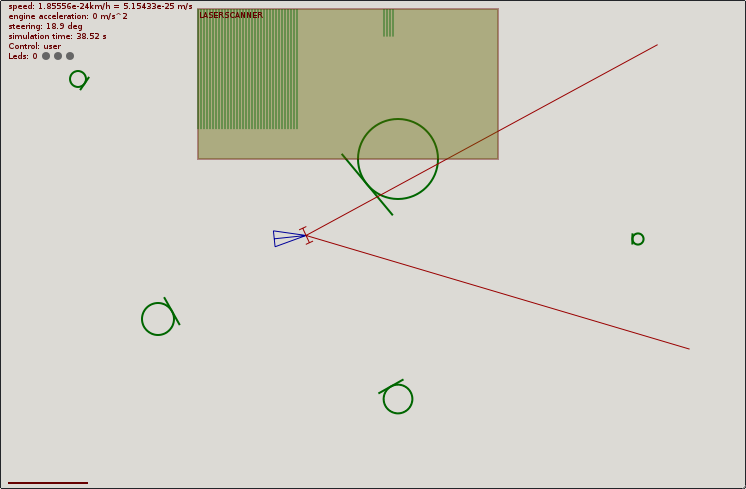
\includegraphics[width=15cm]{pic/sim.png}
\end{center}
\caption{Simulator}
\label{figsim}
\end{figure}




\section{Lessons learned}
%%TODO
\subsection{Electical systems}
\begin{wrapfigure}{r}{0.5\textwidth}
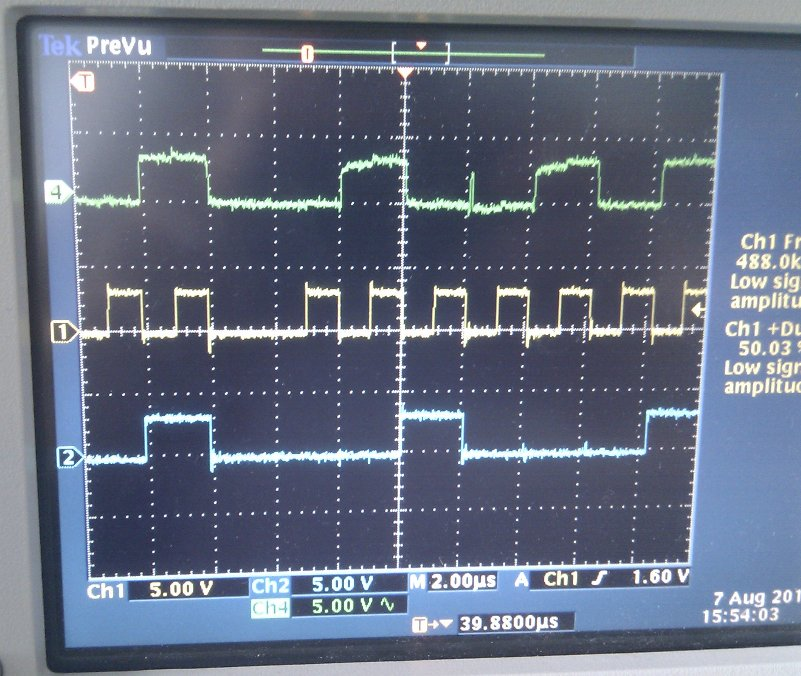
\includegraphics[width=0.48\textwidth]{pic/spi.png}
\caption{Noise on clock causes state machine to fail}
\label{figsim}
\end{wrapfigure}
clock kann rauschen/ungewollte peaks geben
oszi unvermeidlich beim debuggen von kommunikationsprotokollen
trick: debugpin rauslegen und mit dem oszi mitlesen
\subsection{Debugging hardware}
die 7-segmentanzeigen sind nützlich und einfach anzusteuern
Endianness bei kommunikation verschiedener Systeme beachten
\subsection{Safety}
Robots are dangerous! If you make an error in motor control logic engines can start and stop unexpected. 
\begin{wrapfigure}{r}{0.3\textwidth}
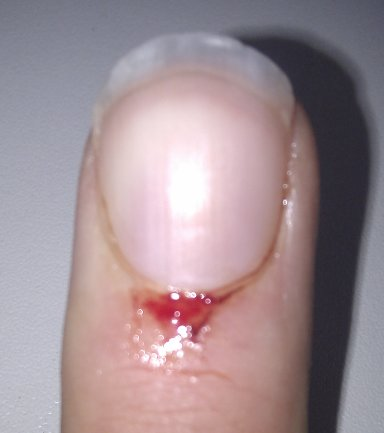
\includegraphics[width=0.29\textwidth]{pic/finger.png}
\caption{Injury due to car}
\label{figsim}
\end{wrapfigure}




lego-connectors sind gut um sachen zu mounten




\section{Conclusions}\label{conclusions}
We worked hard, and achieved very little.

\section{Future work}

\end{document}
